%%____________________________________________________________________________||
\section{Interpretations with simplified ``split SUSY'' models}
\label{app:LLP}

\subsection{Kinematic distributions}
\label{app:LLP-distributions}

Figure \ref{fig:T1qqqqLLvsT1qqqqLL} shows a comparison of the
distributions of the main kinematic variables used for signal
extraction (\njet, \nb, \scalht, and \mht) for various \ctau
models. In general, the distributions become softer with increasing
lifetime, which can be attributed mainly to reduced acceptance to the
jets from the gluino decay with increasing gluino lifetime, with a
higher probability to decay outside the detector, and an increased
reliance on jets from ISR. 

It is also noteworthy that an enhancement in the number of displaced
jets that are b-tagged when \ctau is of order 1~mm. However, this
enhancement is less noticeable for compressed models as the displaced
jets are softer and therefore more likely to be below the jet \pt
threshold.

Figure \ref{fig:T1qqqqLLvsT1qqqq} shows a comparison of the kinematic
distributions between the ``standard'' simplified \texttt{T1qqqq}
model that assumes the prompt decay of gluinos (with the detector
response from \texttt{FastSim}) and the \texttt{T1qqqqLL} model with a
``prompt-like'' lifetime of $\ctau = 0.001\unit{mm}$ (with the
detector response from \texttt{FullSim}).  The two samples show
reasonable agreement.

Similarly, Fig.~\ref{fig:T1qqqqLLvsT1bbbb} shows a comparison of
kinematic distributions for the ``standard'' simplified
\texttt{T1bbbb} model (\texttt{FastSim}) and the \texttt{T1qqqqLL}
model with $\ctau = 1\unit{mm}$ model (\texttt{FullSim}). The two
models exhibit similar kinematical behaviours. There are some
differences in the \nb distribution that arise from the differences in
the b-tagging efficiencies for displaced jets and genuine b-jets that
grow as a function of jet \pt, as shown in
Sec.~\ref{app:LLP-btagging}, and is thus more noticeable for the
compressed samples.

\begin{figure}[h!]
  \begin{center}
    \subfigure{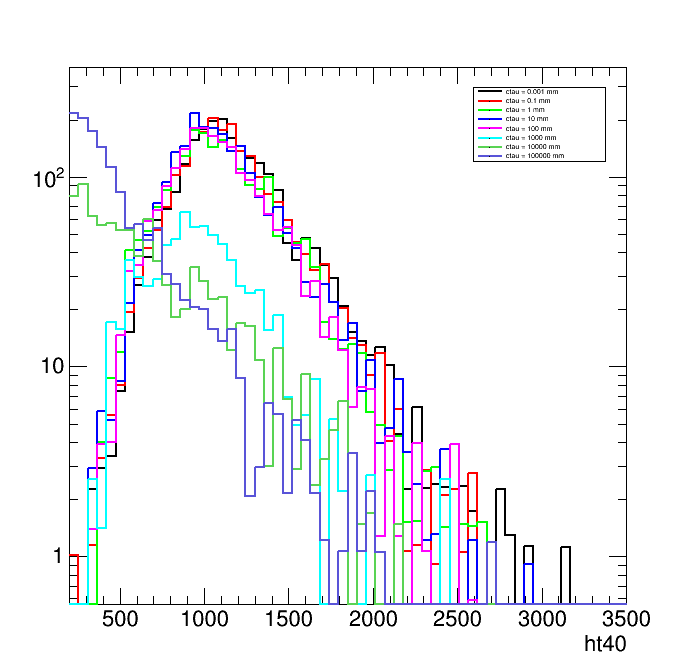
\includegraphics[width=0.28\textwidth]{figures/LLPResults/T1qqqqLL_1000_200/ht40_all_all}} ~
    \subfigure{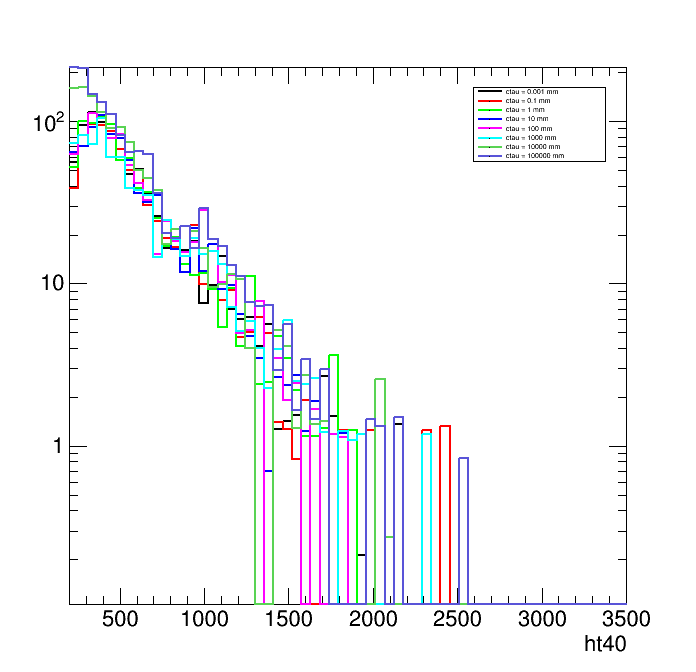
\includegraphics[width=0.28\textwidth]{figures/LLPResults/T1qqqqLL_1000_900/ht40_all_all}} \\
    \subfigure{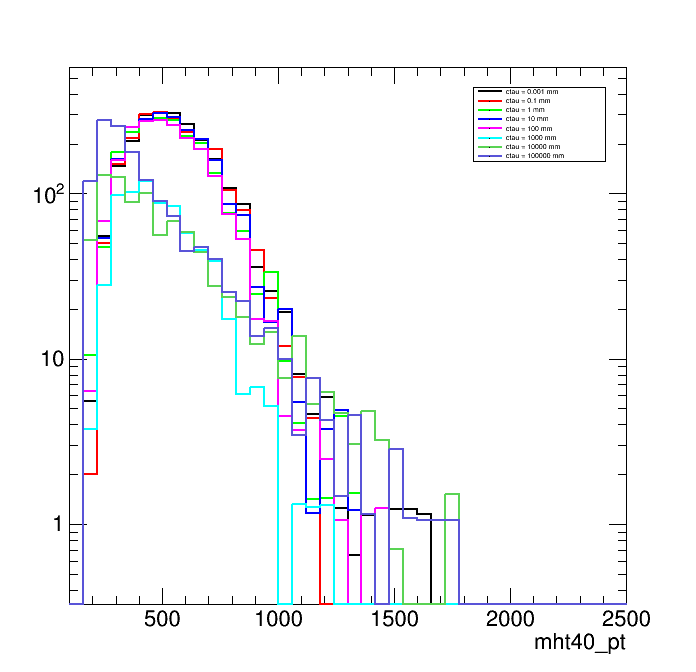
\includegraphics[width=0.28\textwidth]{figures/LLPResults/T1qqqqLL_1000_200/mht40_pt_all_all}} ~
    \subfigure{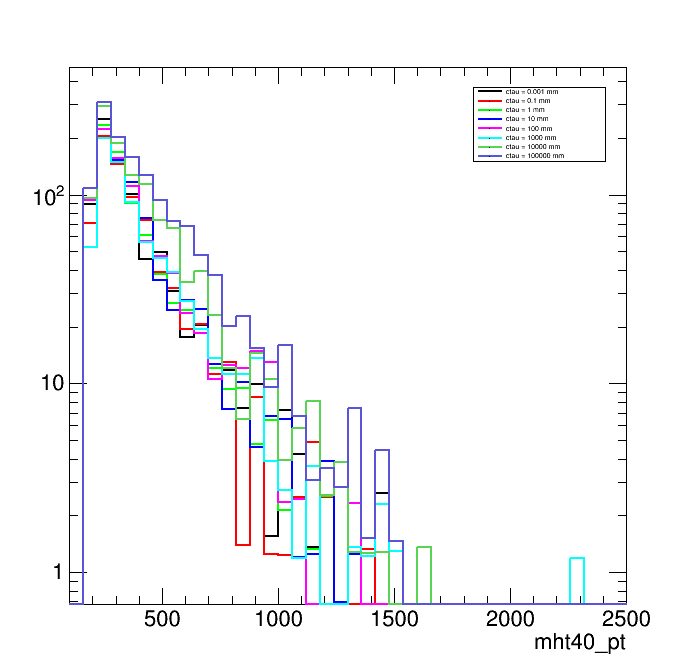
\includegraphics[width=0.28\textwidth]{figures/LLPResults/T1qqqqLL_1000_900/mht40_pt_all_all}} \\
    \subfigure{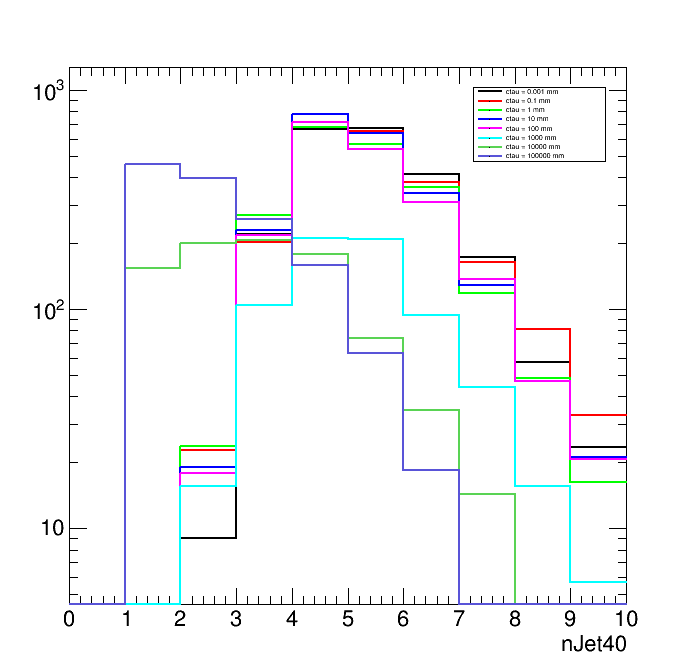
\includegraphics[width=0.28\textwidth]{figures/LLPResults/T1qqqqLL_1000_200/nJet40_all_all}} ~
    \subfigure{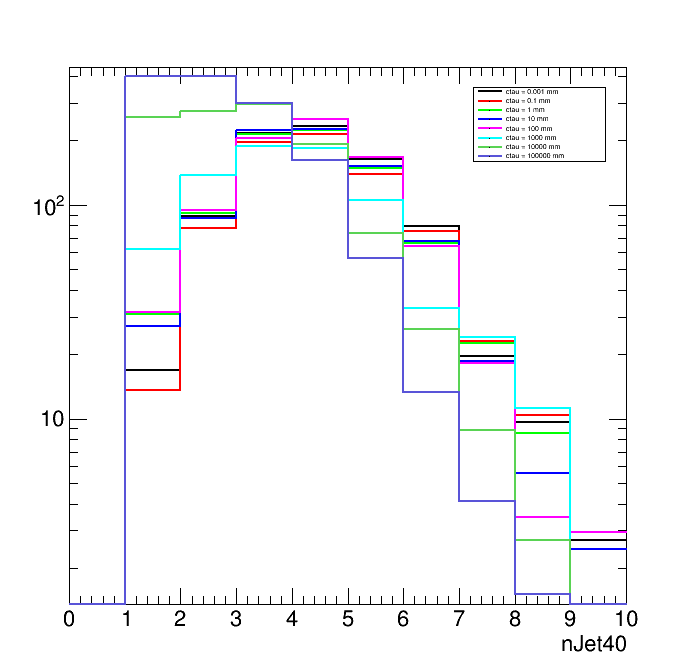
\includegraphics[width=0.28\textwidth]{figures/LLPResults/T1qqqqLL_1000_900/nJet40_all_all}} \\
    \subfigure{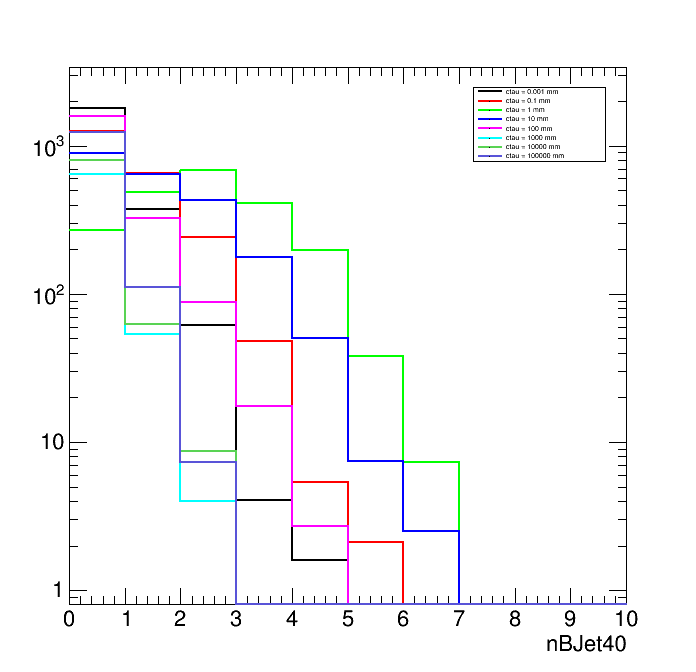
\includegraphics[width=0.28\textwidth]{figures/LLPResults/T1qqqqLL_1000_200/nBJet40_all_all}} ~
    \subfigure{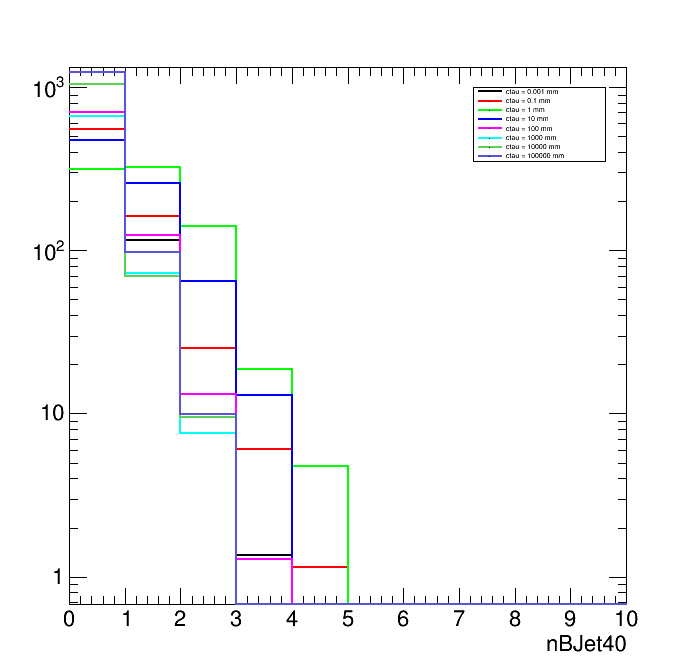
\includegraphics[width=0.28\textwidth]{figures/LLPResults/T1qqqqLL_1000_900/nBJet40_all_all}}
    \caption{Kinematic distributions comparing various gluino
      lifetimes, for an uncompressed (1000,200) (Left) and compressed
      (1000,900) (Right) mass point.}
    \label{fig:T1qqqqLLvsT1qqqqLL}
  \end{center}
\end{figure}

\begin{figure}[h!]
  \begin{center}
    \subfigure{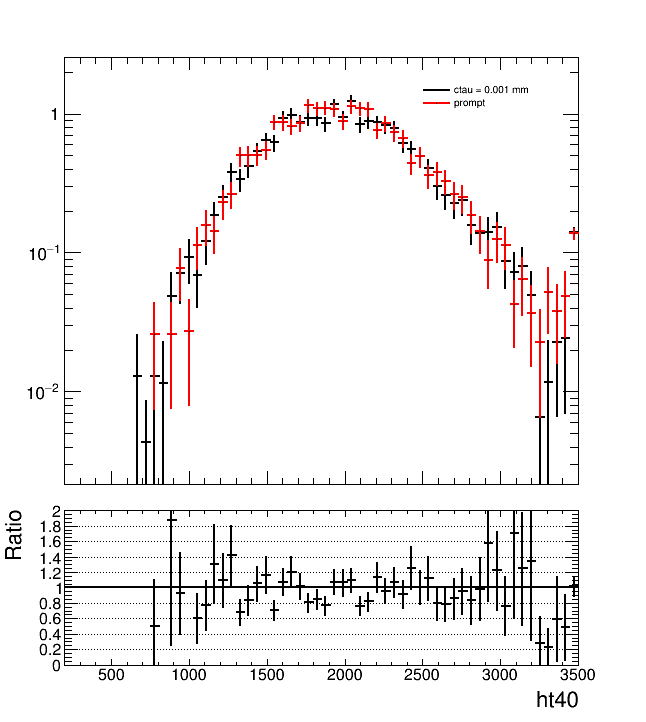
\includegraphics[width=0.28\textwidth]{figures/LLPResults/T1qqqqLL_vs_T1qqqq_1800_200/ht40_all_all}} ~
    \subfigure{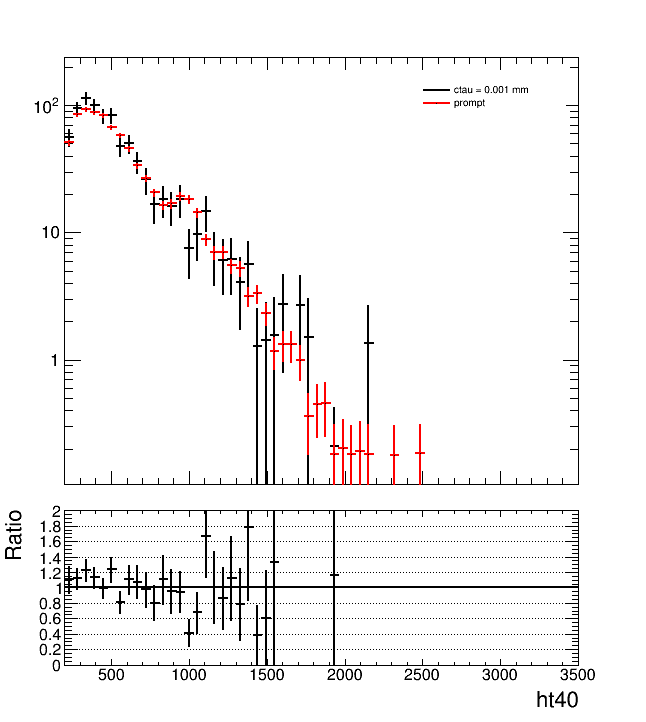
\includegraphics[width=0.28\textwidth]{figures/LLPResults/T1qqqqLL_vs_T1qqqq_1000_900/ht40_all_all}} \\
    \subfigure{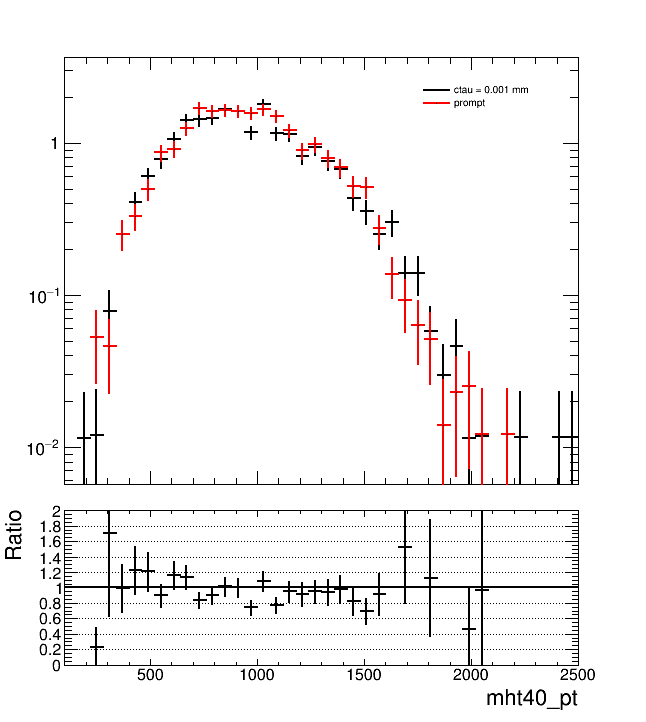
\includegraphics[width=0.28\textwidth]{figures/LLPResults/T1qqqqLL_vs_T1qqqq_1800_200/mht40_pt_all_all}} ~
    \subfigure{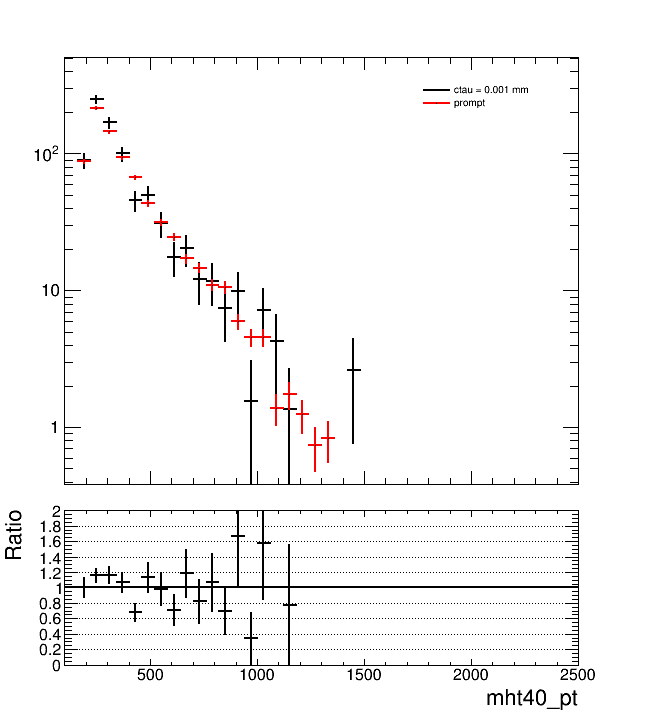
\includegraphics[width=0.28\textwidth]{figures/LLPResults/T1qqqqLL_vs_T1qqqq_1000_900/mht40_pt_all_all}} \\
    \subfigure{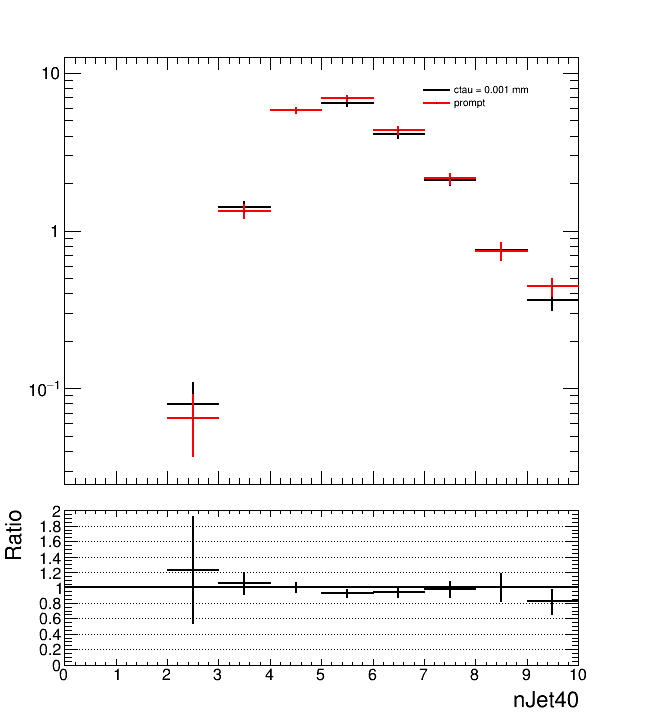
\includegraphics[width=0.28\textwidth]{figures/LLPResults/T1qqqqLL_vs_T1qqqq_1800_200/nJet40_all_all}} ~
    \subfigure{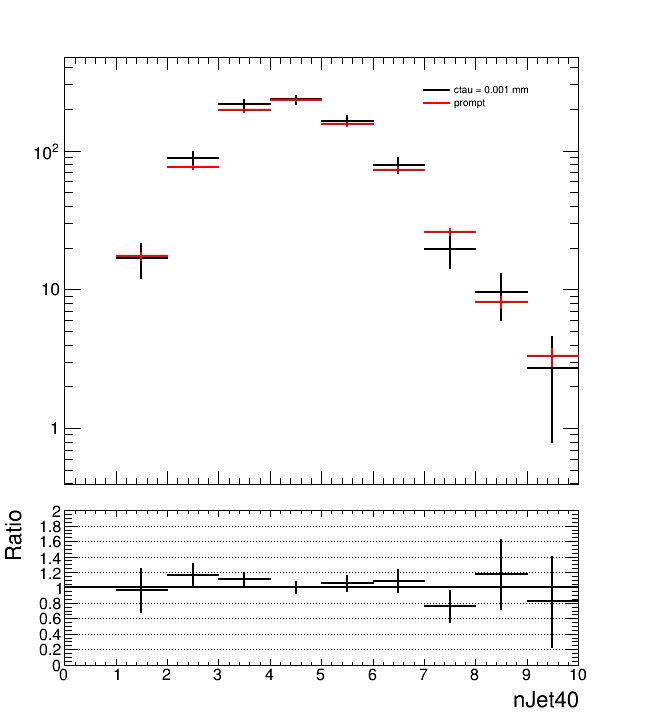
\includegraphics[width=0.28\textwidth]{figures/LLPResults/T1qqqqLL_vs_T1qqqq_1000_900/nJet40_all_all}} \\
    \subfigure{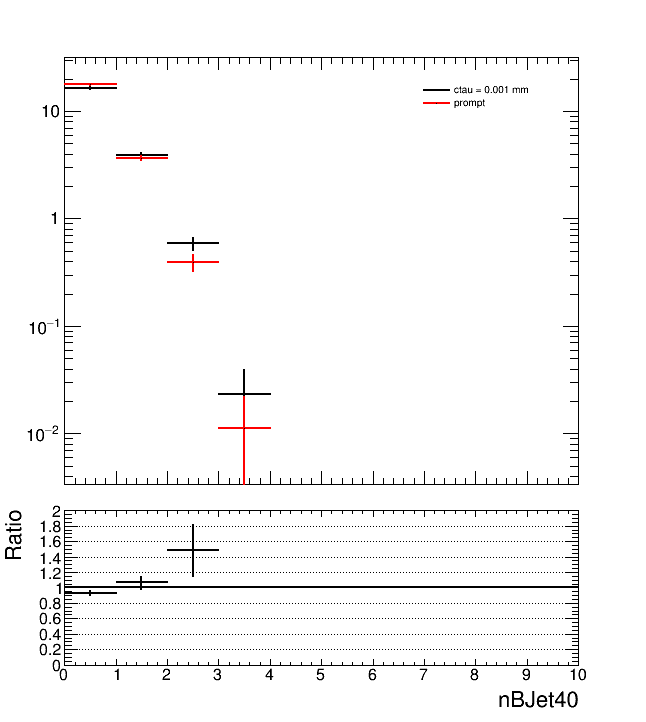
\includegraphics[width=0.28\textwidth]{figures/LLPResults/T1qqqqLL_vs_T1qqqq_1800_200/nBJet40_all_all}} ~
    \subfigure{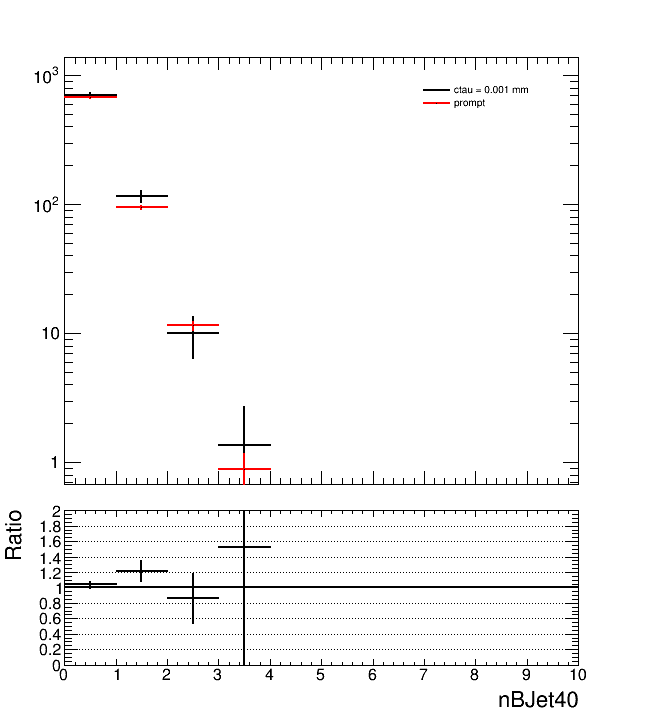
\includegraphics[width=0.28\textwidth]{figures/LLPResults/T1qqqqLL_vs_T1qqqq_1000_900/nBJet40_all_all}}
    \caption{Kinematic distributions comparing prompt T1qqqq and
      T1qqqqLL with $\ctau = 0.001\unit{mm}$, for an uncompressed
      (1800,200) (Left) and compressed (1000,900) (Right) mass point.}
    \label{fig:T1qqqqLLvsT1qqqq}
  \end{center}
\end{figure}

\begin{figure}[h!]
  \begin{center}
    \subfigure{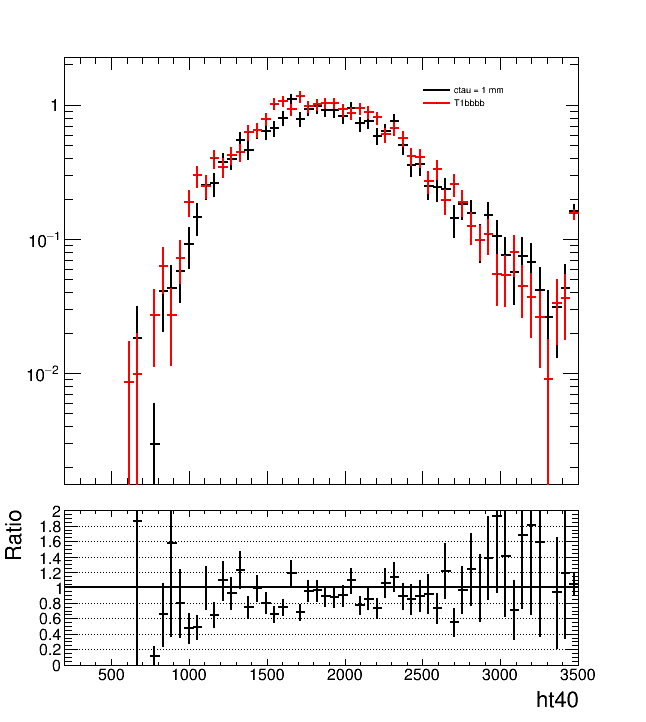
\includegraphics[width=0.28\textwidth]{figures/LLPResults/T1qqqqLL_vs_T1bbbb_1800_200/ht40_all_all}} ~
    \subfigure{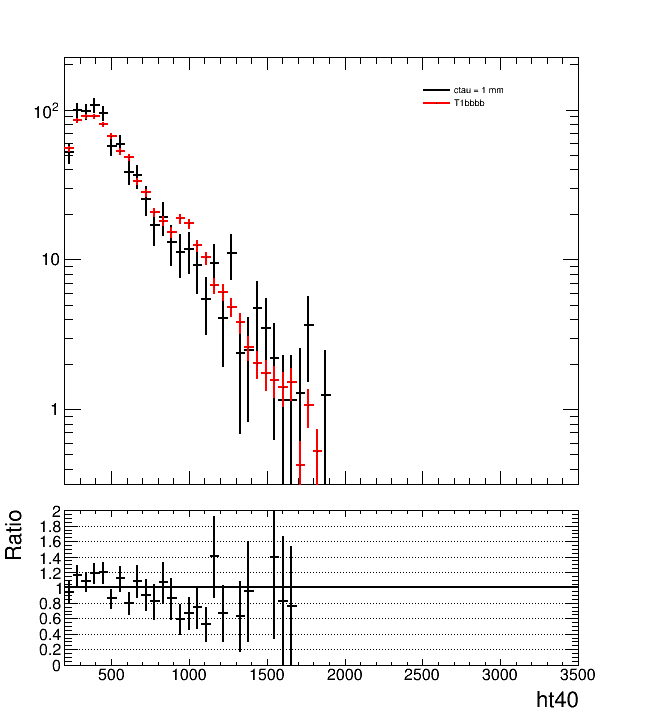
\includegraphics[width=0.28\textwidth]{figures/LLPResults/T1qqqqLL_vs_T1bbbb_1000_900/ht40_all_all}} \\
    \subfigure{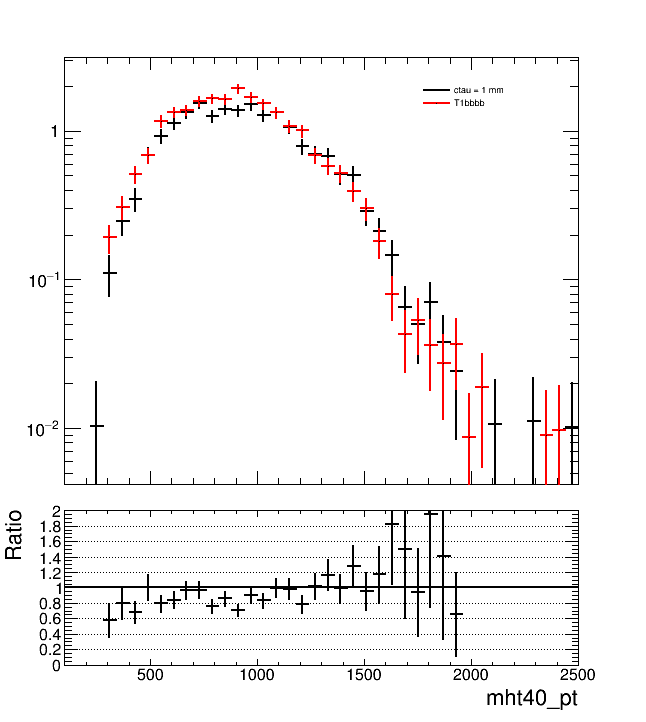
\includegraphics[width=0.28\textwidth]{figures/LLPResults/T1qqqqLL_vs_T1bbbb_1800_200/mht40_pt_all_all}} ~
    \subfigure{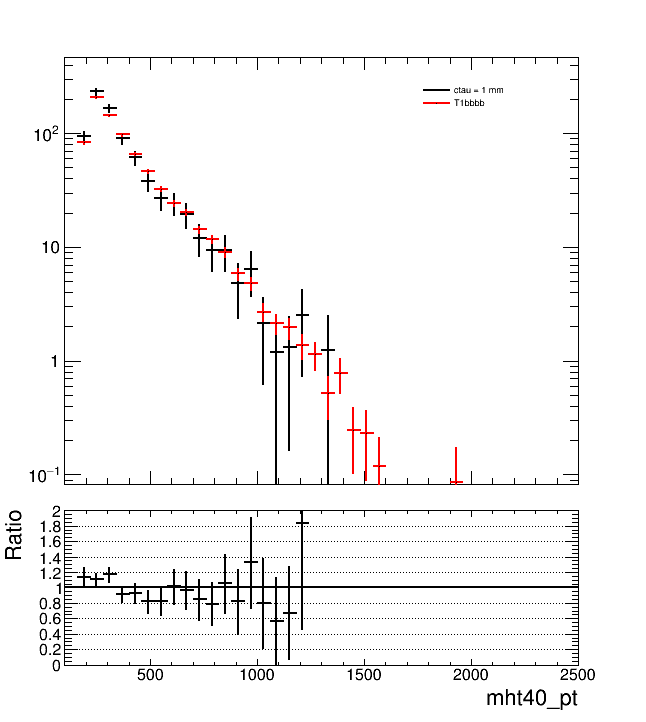
\includegraphics[width=0.28\textwidth]{figures/LLPResults/T1qqqqLL_vs_T1bbbb_1000_900/mht40_pt_all_all}} \\
    \subfigure{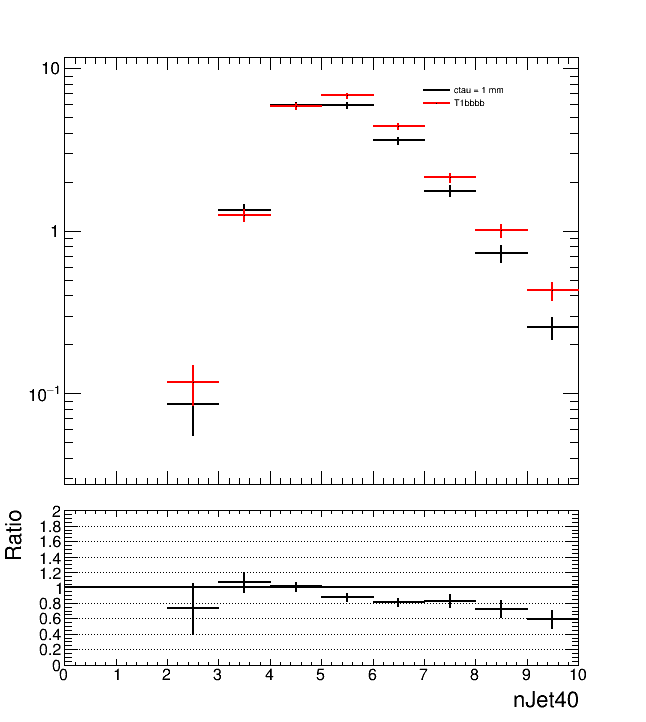
\includegraphics[width=0.28\textwidth]{figures/LLPResults/T1qqqqLL_vs_T1bbbb_1800_200/nJet40_all_all}} ~
    \subfigure{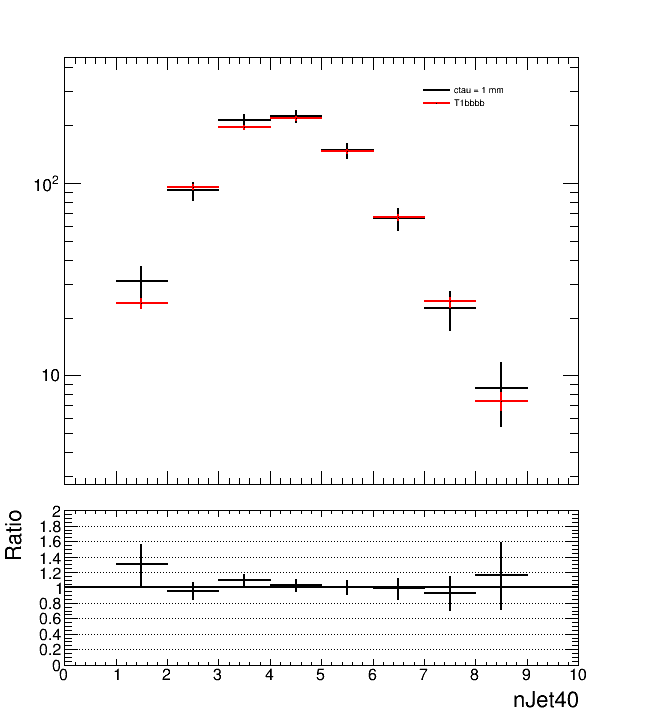
\includegraphics[width=0.28\textwidth]{figures/LLPResults/T1qqqqLL_vs_T1bbbb_1000_900/nJet40_all_all}} \\
    \subfigure{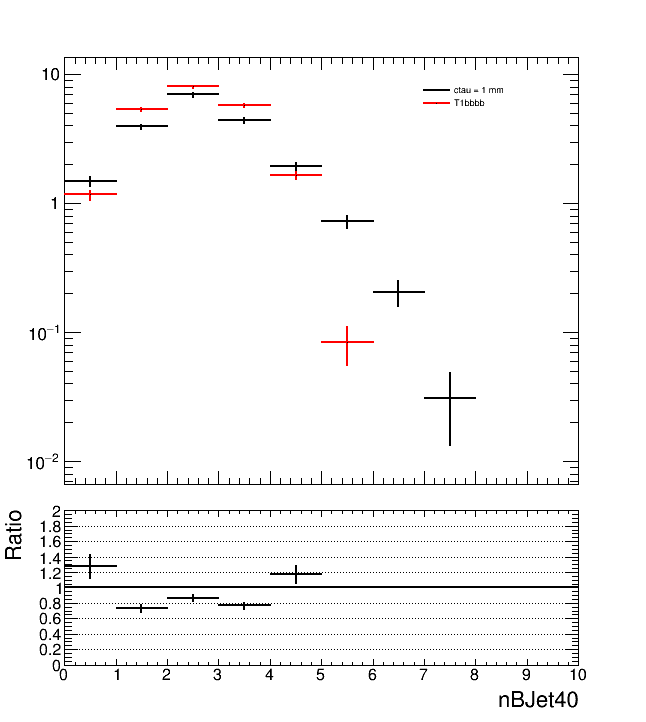
\includegraphics[width=0.28\textwidth]{figures/LLPResults/T1qqqqLL_vs_T1bbbb_1800_200/nBJet40_all_all}} ~
    \subfigure{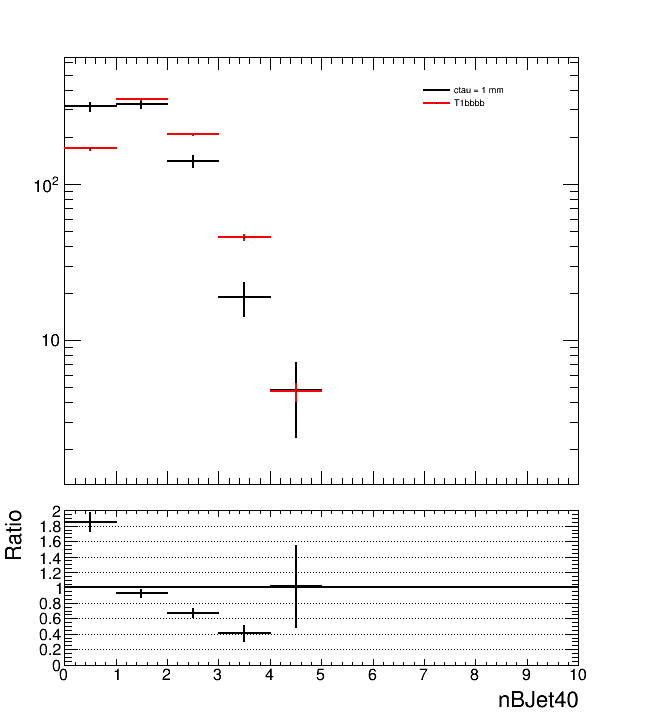
\includegraphics[width=0.28\textwidth]{figures/LLPResults/T1qqqqLL_vs_T1bbbb_1000_900/nBJet40_all_all}}
    \caption{Kinematic distributions comparing prompt T1bbbb and
      T1qqqqLL with $\ctau = 1\unit{mm}$, for an uncompressed
      (1800,200) (Left) and compressed (1000,900) (Right) mass point.}
    \label{fig:T1qqqqLLvsT1bbbb}
  \end{center}
\end{figure}

\clearpage
\subsection{Signal efficiencies related jet ID}
\label{app:LLP-jetid}

Table~\ref{tab:LLP-chf} shows the signal efficiency for the $0.1 <
\text{CHF} < 0.95$ requirement on the lead jet (described in
Sec.~\ref{sec:chf}) for the \texttt{T1qqqqLL} (1800,200), (1000,200),
and (1000,900) benchmark models and as a function of gluino lifetime,
$c\tau$, following all other selections except the odd jet veto
requirement discussed below. ``Representative'' efficiences as a
function of $c\tau$ are also shown when integrating over all models in
terms of masses.  Generally, the efficiency is 100\%, but falls to
${\approx}30\%$ for models with $c\tau \approx 10^{3} -
10^{4}\unit{mm}$ when experimental acceptance relies on displaced jets
with vertices in the range $\approx 0.1-10\unit{m}$.\footnote{This
  range of displacements covers the outermost barrel layer of the
  pixel system to the outermost barrel layer of the muon system.}

Table~\ref{tab:LLP-oddjetveto} shows the signal efficiency for the odd
jet veto (described in Sec.~\ref{sec:jetsacc}) for the
\texttt{T1qqqqLL} (1800,200), (1000,200), and (1000,900) benchmark
models and as a function of gluino lifetime, $c\tau$, following all
other selections. ``Representative'' efficiences as a function of
$c\tau$ are also shown when integrating over all models in terms of
masses.  Generally, the efficiency is 100\%, but falls to
${\approx}90\%$ for models with $c\tau \approx 10^{3} -
10^{4}\unit{mm}$ when experimental acceptance relies on displaced jets
with vertices in the range $\approx 0.1-10\unit{m}$. Systematic
uncertainties in the odd jet veto are assumed to be equal to the size
of the inefficiency, \ie in the range 0--10\%.

Figure~\ref{fig:oddjetveto} shows the signal efficiency for the odd
jet veto as a function of the flight distances of the each gluino in
the event for the simplified \texttt{T1qqqqLL} model for a range of
gluino lifetimes and the range $10 < \ctau <
100000\unit{mm}$. Inefficiencies tend to be localised to flight
distances of either or both gluinos in the region from
${\approx}100\unit{mm}$ to ${\approx}10\unit{m}$, as best indicated by
Figure~\ref{fig:oddjetveto} (bottom right), which shows
``representative'' efficiences when integrating over all models in
terms of masses and $c\tau$ values.

\clearpage
\begin{table}[h!]
  \topcaption{Summary of the signal efficiencies for the CHF
    requirement on the lead-\pt jet in the event for three
    \texttt{T1qqqqLL} benchmark models ($m_\text{gluino},
    m_\text{LSP}$), as a function of $c\tau$. Also shown are
    ``representative'' efficiences when integrating over all masses.}  
  \centering
  \begin{tabular}{lcccc} 
    \hline
    $c\tau$          & \multicolumn{4}{c}{Efficiency [\%]}               \\
    \cline{2-5}
                     & (1800,200) & (1000,200) & (1000,900) & All masses \\
    \hline
    $0.001\unit{mm}$ & 98.9       & 99.2       & 99.4       & --         \\
%    $0.01\unit{mm}$ & 100.0      & 100.0      & 100.0      & 100.0      \\
    $0.1\unit{mm}$   & 99.0       & 98.9       & 99.8       & --         \\
    $1\unit{mm}$     & 97.0       & 97.6       & 99.3       & --         \\
    $10\unit{mm}$    & 94.4       & 96.6       & 99.9       & --         \\
    $100\unit{mm}$   & 81.3       & 86.6       & 99.2       & --         \\
    $1\unit{m}$      & 39.7       & 43.9       & 95.0       & --         \\
    $10\unit{m}$     & 25.4       & 36.4       & 95.1       & --         \\
    $100\unit{m}$    & --         & 80.6       & 98.9       & --         \\
    \hline
  \end{tabular}
  \label{tab:LLP-chf}
\end{table}

\begin{table}[h!]
  \topcaption{Summary of the signal efficiencies for the odd jet veto
    for three \texttt{T1qqqqLL} benchmark models ($m_\text{gluino}, 
    m_\text{LSP}$), as a function of $c\tau$. Also shown are
    ``representative'' efficiences when integrating over all masses.} 
\centering
  \begin{tabular}{lcccc} 
    \hline
    $c\tau$          & \multicolumn{4}{c}{Efficiency [\%]}               \\
    \cline{2-5}
                     & (1800,200) & (1000,200) & (1000,900) & All masses \\
    \hline
    $0.001\unit{mm}$ & 99.9       & 100.0      & 100.0      & 99.6       \\
%    $0.01\unit{mm}$ & 100.0      & 100.0      & 100.0      & 100.0      \\
    $0.1\unit{mm}$   & 99.9       & 100.0      & 99.8       & 99.6       \\
    $1\unit{mm}$     & 99.6       & 100.0      & 99.9       & 99.3       \\
    $10\unit{mm}$    & 99.7       & 99.7       & 100.0      & 99.3       \\
    $100\unit{mm}$   & 99.2       & 98.9       & 99.6       & 98.9       \\
    $1\unit{m}$      & 91.4       & 91.8       & 97.8       & 91.2       \\
    $10\unit{m}$     & 93.8       & 93.8       & 98.0       & 92.8       \\
    $100\unit{m}$    & --         & 99.9       & 99.8       & 99.0       \\
    \hline
  \end{tabular}
  \label{tab:LLP-oddjetveto}
\end{table}

\begin{figure}[h!]
  \begin{center}
%    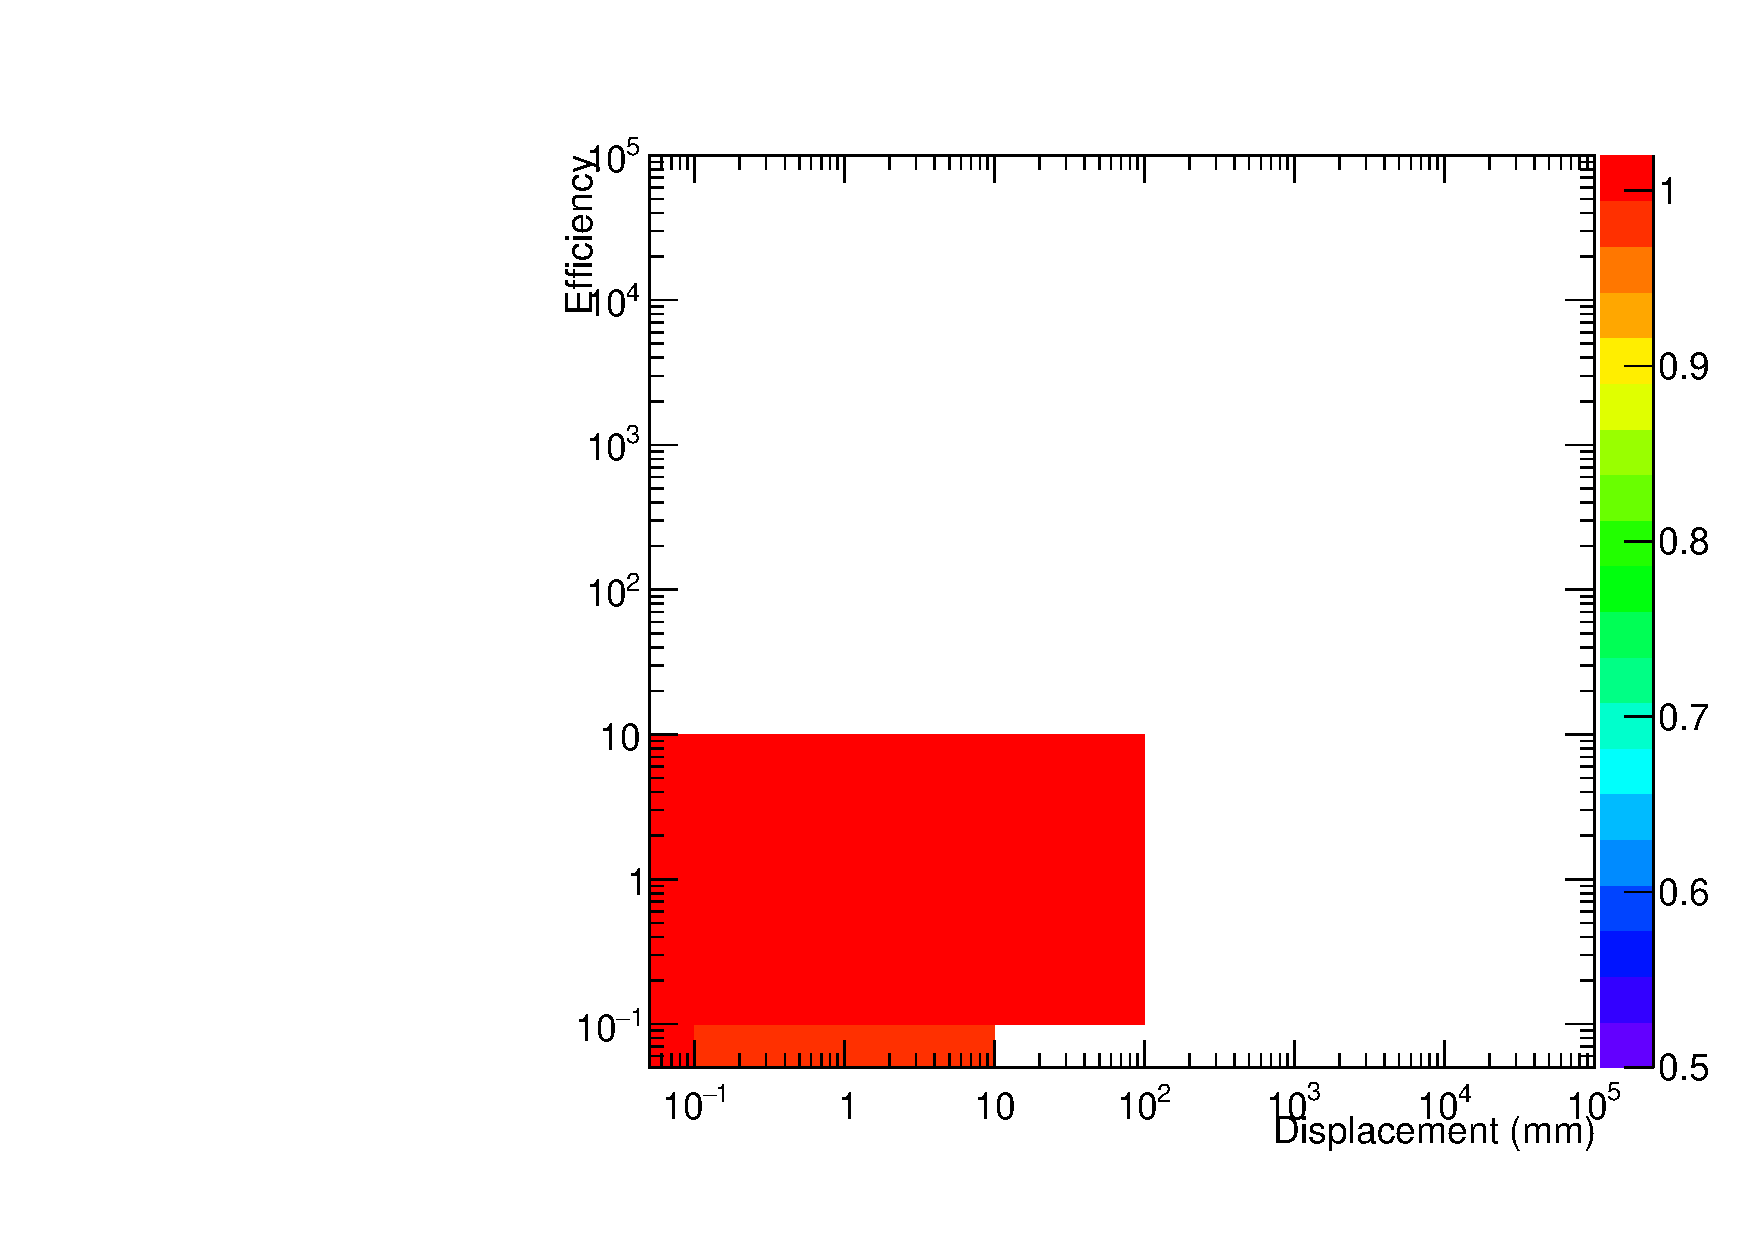
\includegraphics[width=0.4\textwidth]{figures/LLPResults/systs/oddjetveto/Signal_SignalModels__longLivedAnalyzer__SMS-T1qqqqLL_ctau_1_mGluino-1000_mLSP-200_25ns__eff_oddjet_2D_log_num.pdf} 
    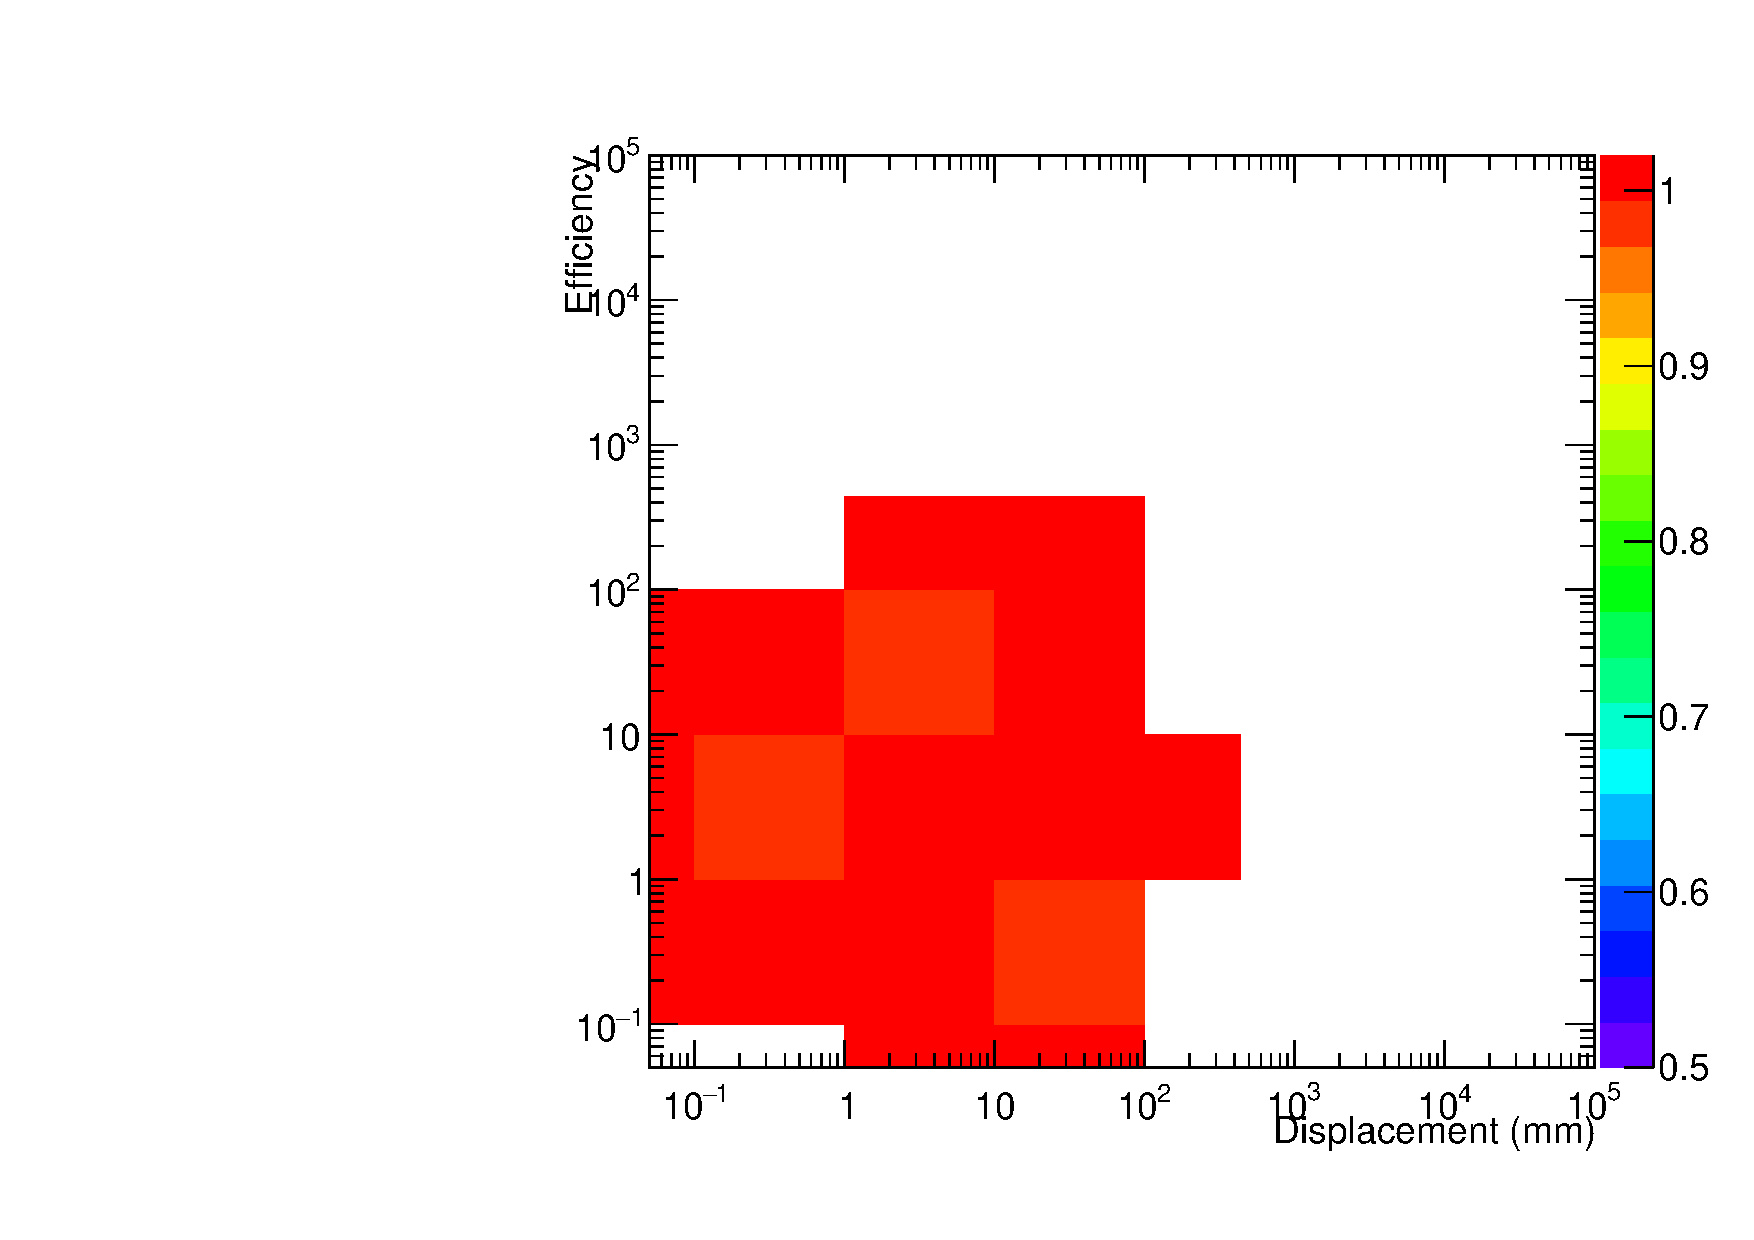
\includegraphics[width=0.4\textwidth]{figures/LLPResults/systs/oddjetveto/Signal_SignalModels__longLivedAnalyzer__SMS-T1qqqqLL_ctau_10_mGluino-1000_mLSP-200_25ns__eff_oddjet_2D_log_num.pdf} 
    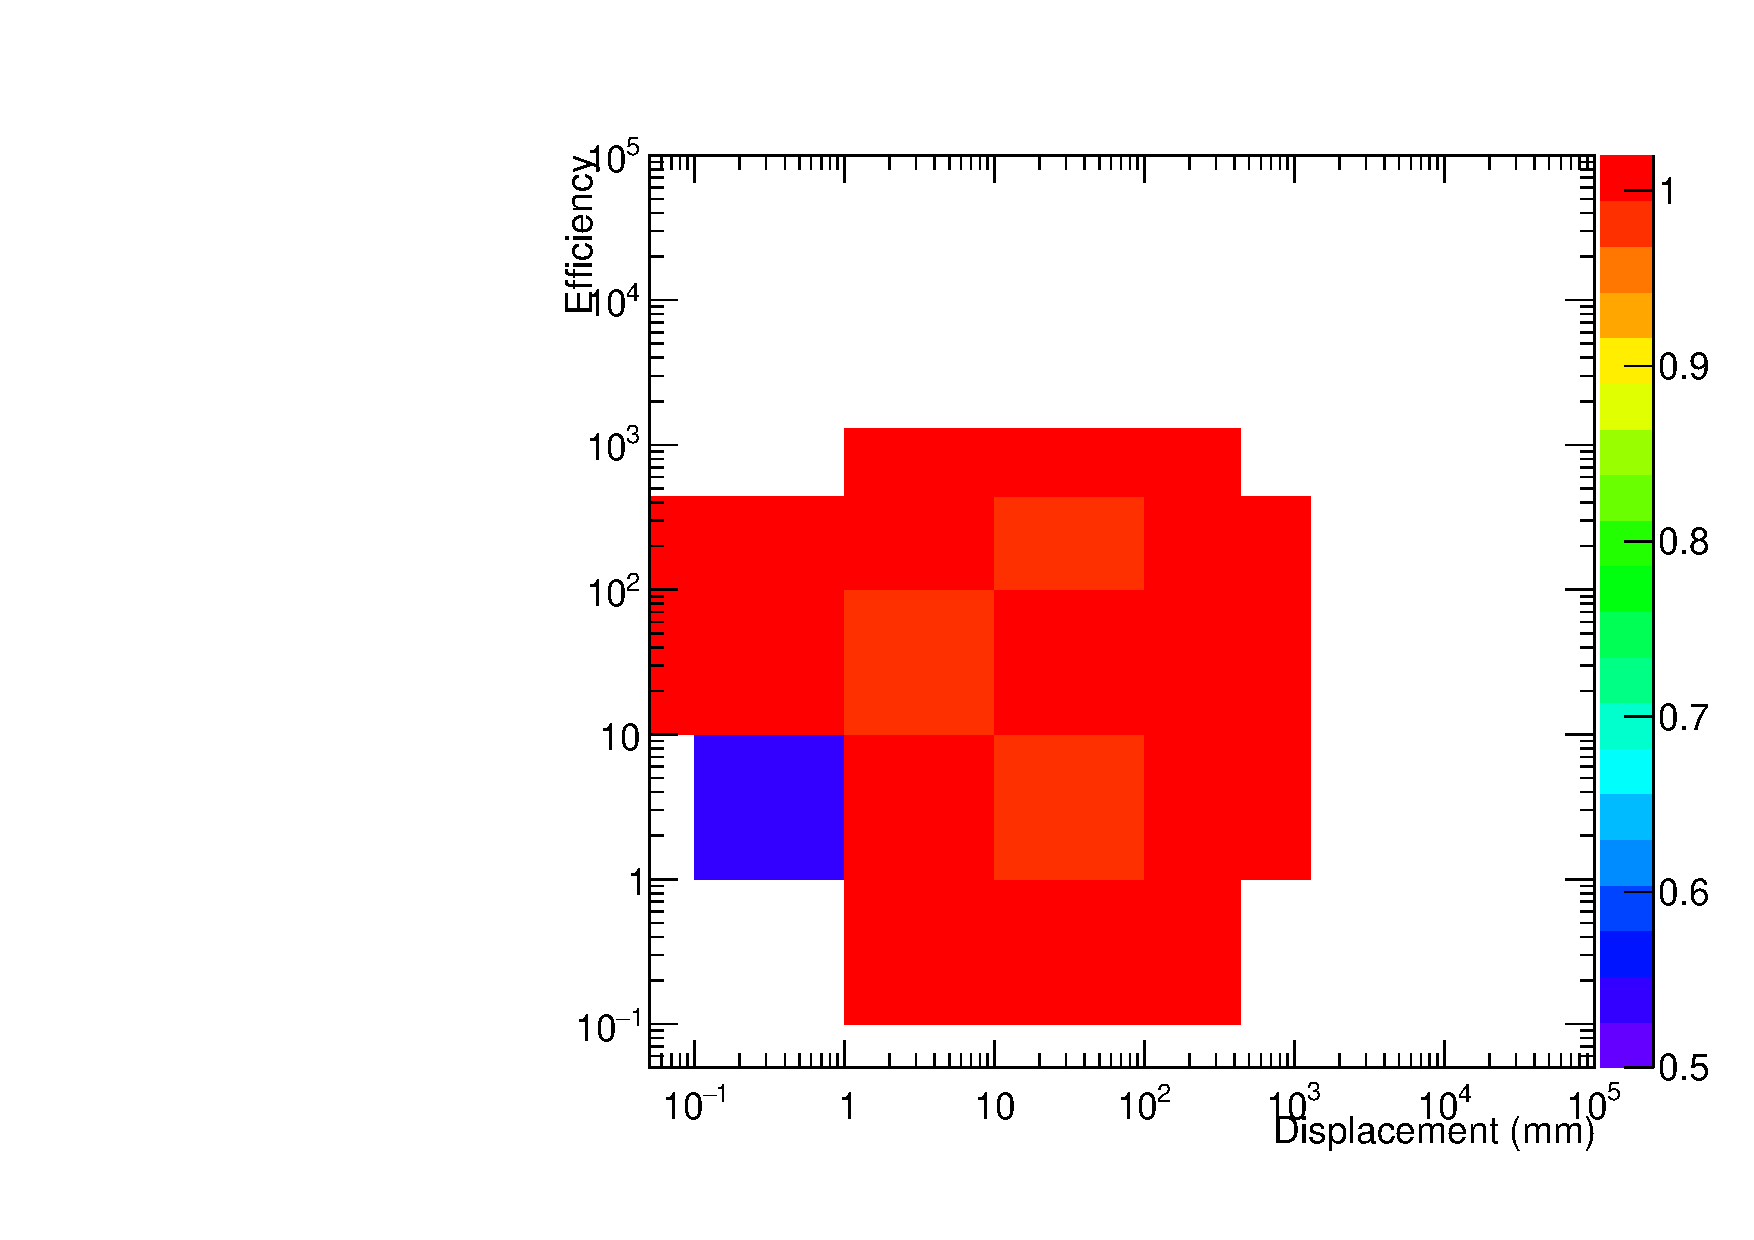
\includegraphics[width=0.4\textwidth]{figures/LLPResults/systs/oddjetveto/Signal_SignalModels__longLivedAnalyzer__SMS-T1qqqqLL_ctau_100_mGluino-1000_mLSP-200_25ns__eff_oddjet_2D_log_num.pdf} \\
    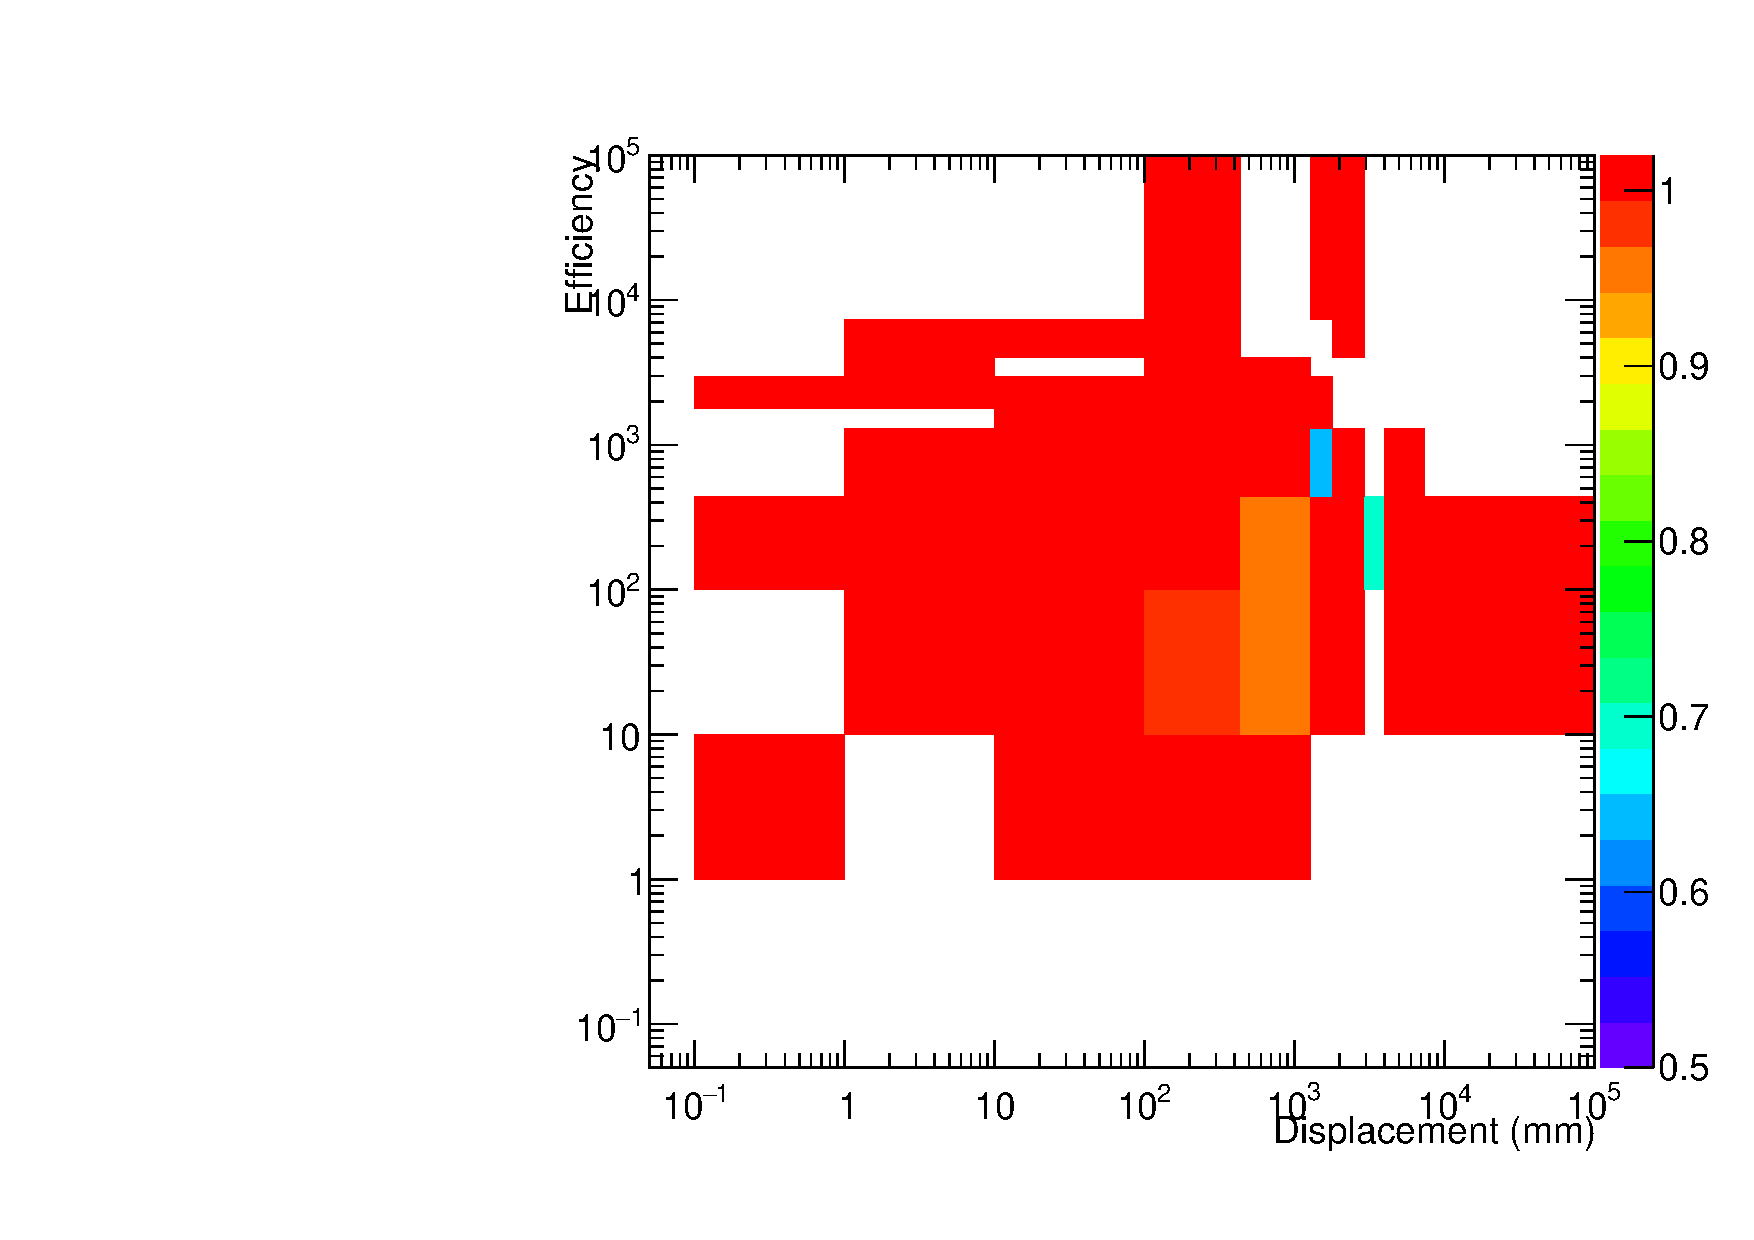
\includegraphics[width=0.4\textwidth]{figures/LLPResults/systs/oddjetveto/Signal_SignalModels__longLivedAnalyzer__SMS-T1qqqqLL_ctau_1000_mGluino-1000_mLSP-200_25ns__eff_oddjet_2D_log_num.pdf} 
    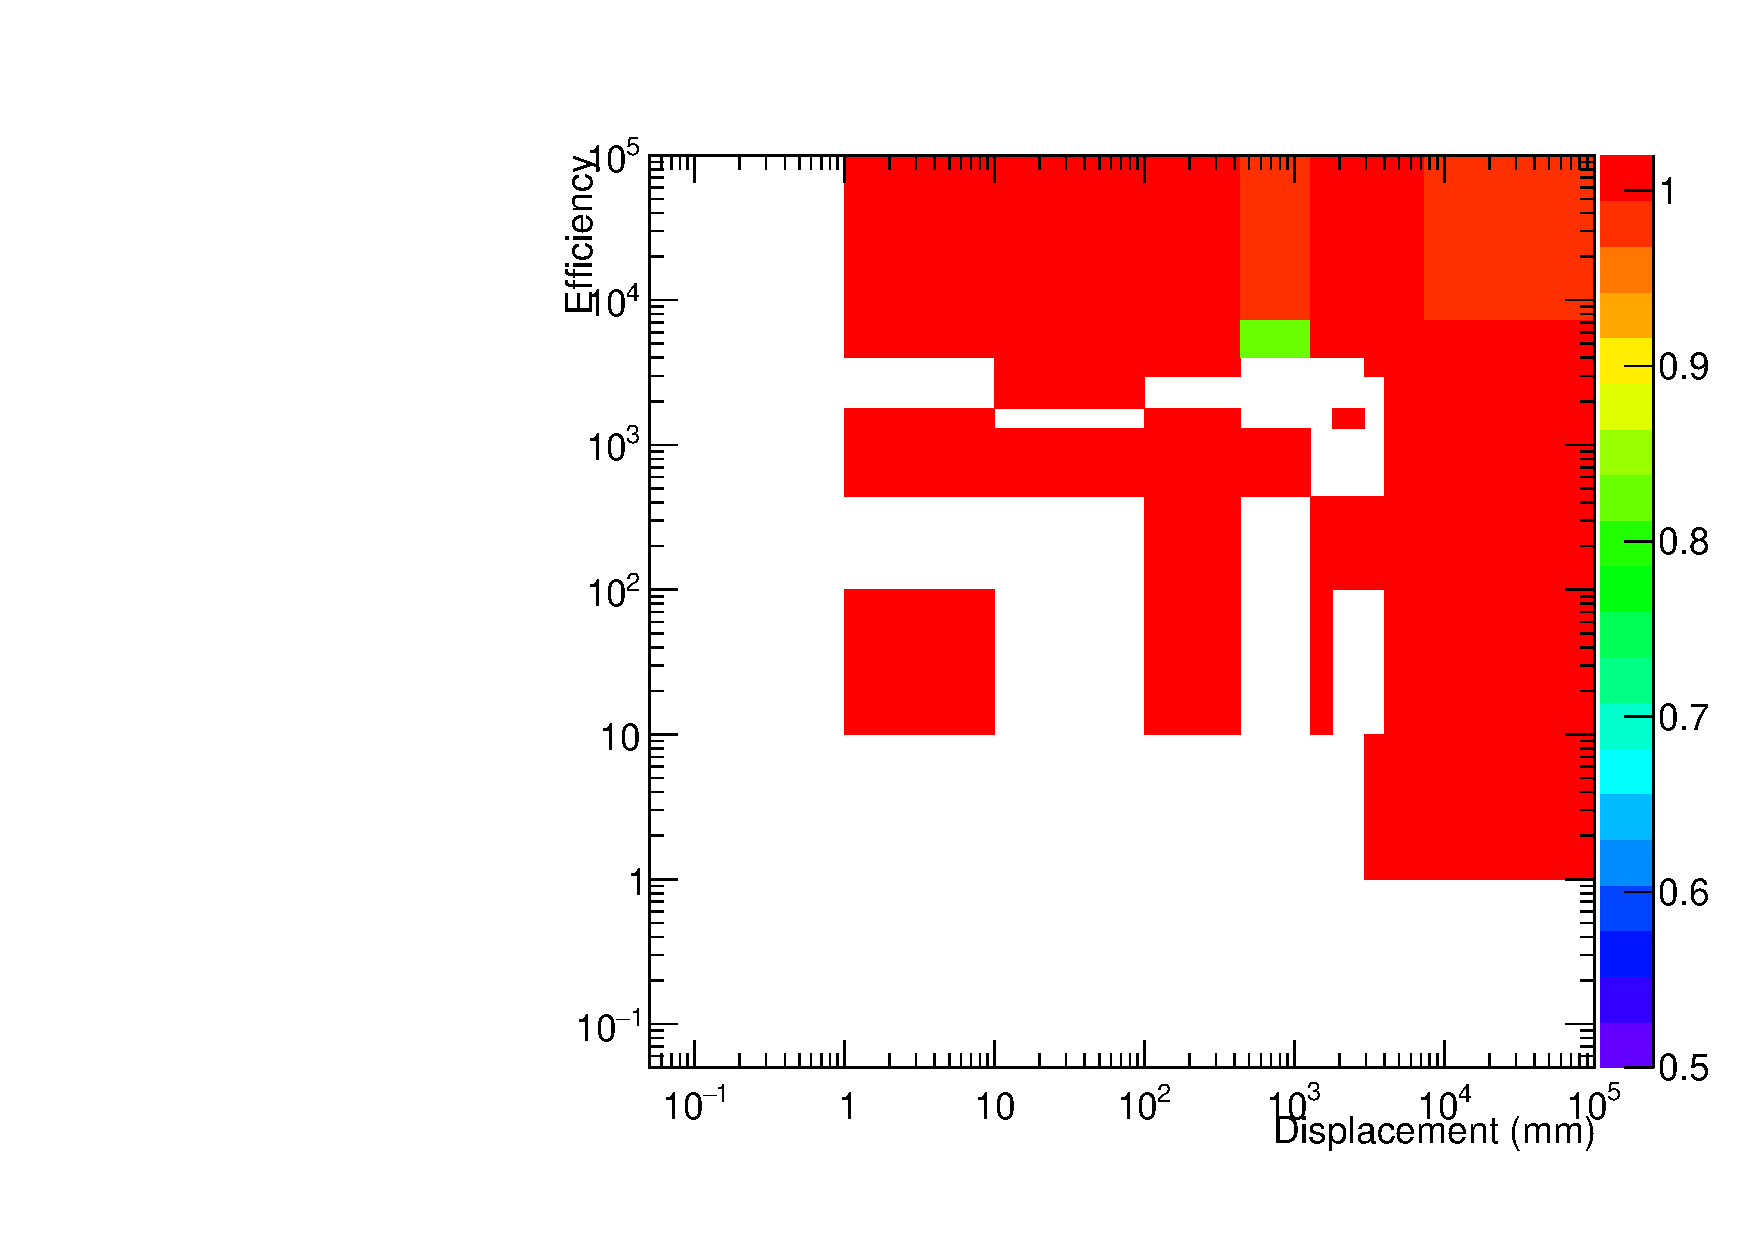
\includegraphics[width=0.4\textwidth]{figures/LLPResults/systs/oddjetveto/Signal_SignalModels__longLivedAnalyzer__SMS-T1qqqqLL_ctau_10000_mGluino-1000_mLSP-200_25ns__eff_oddjet_2D_log_num.pdf} \\
    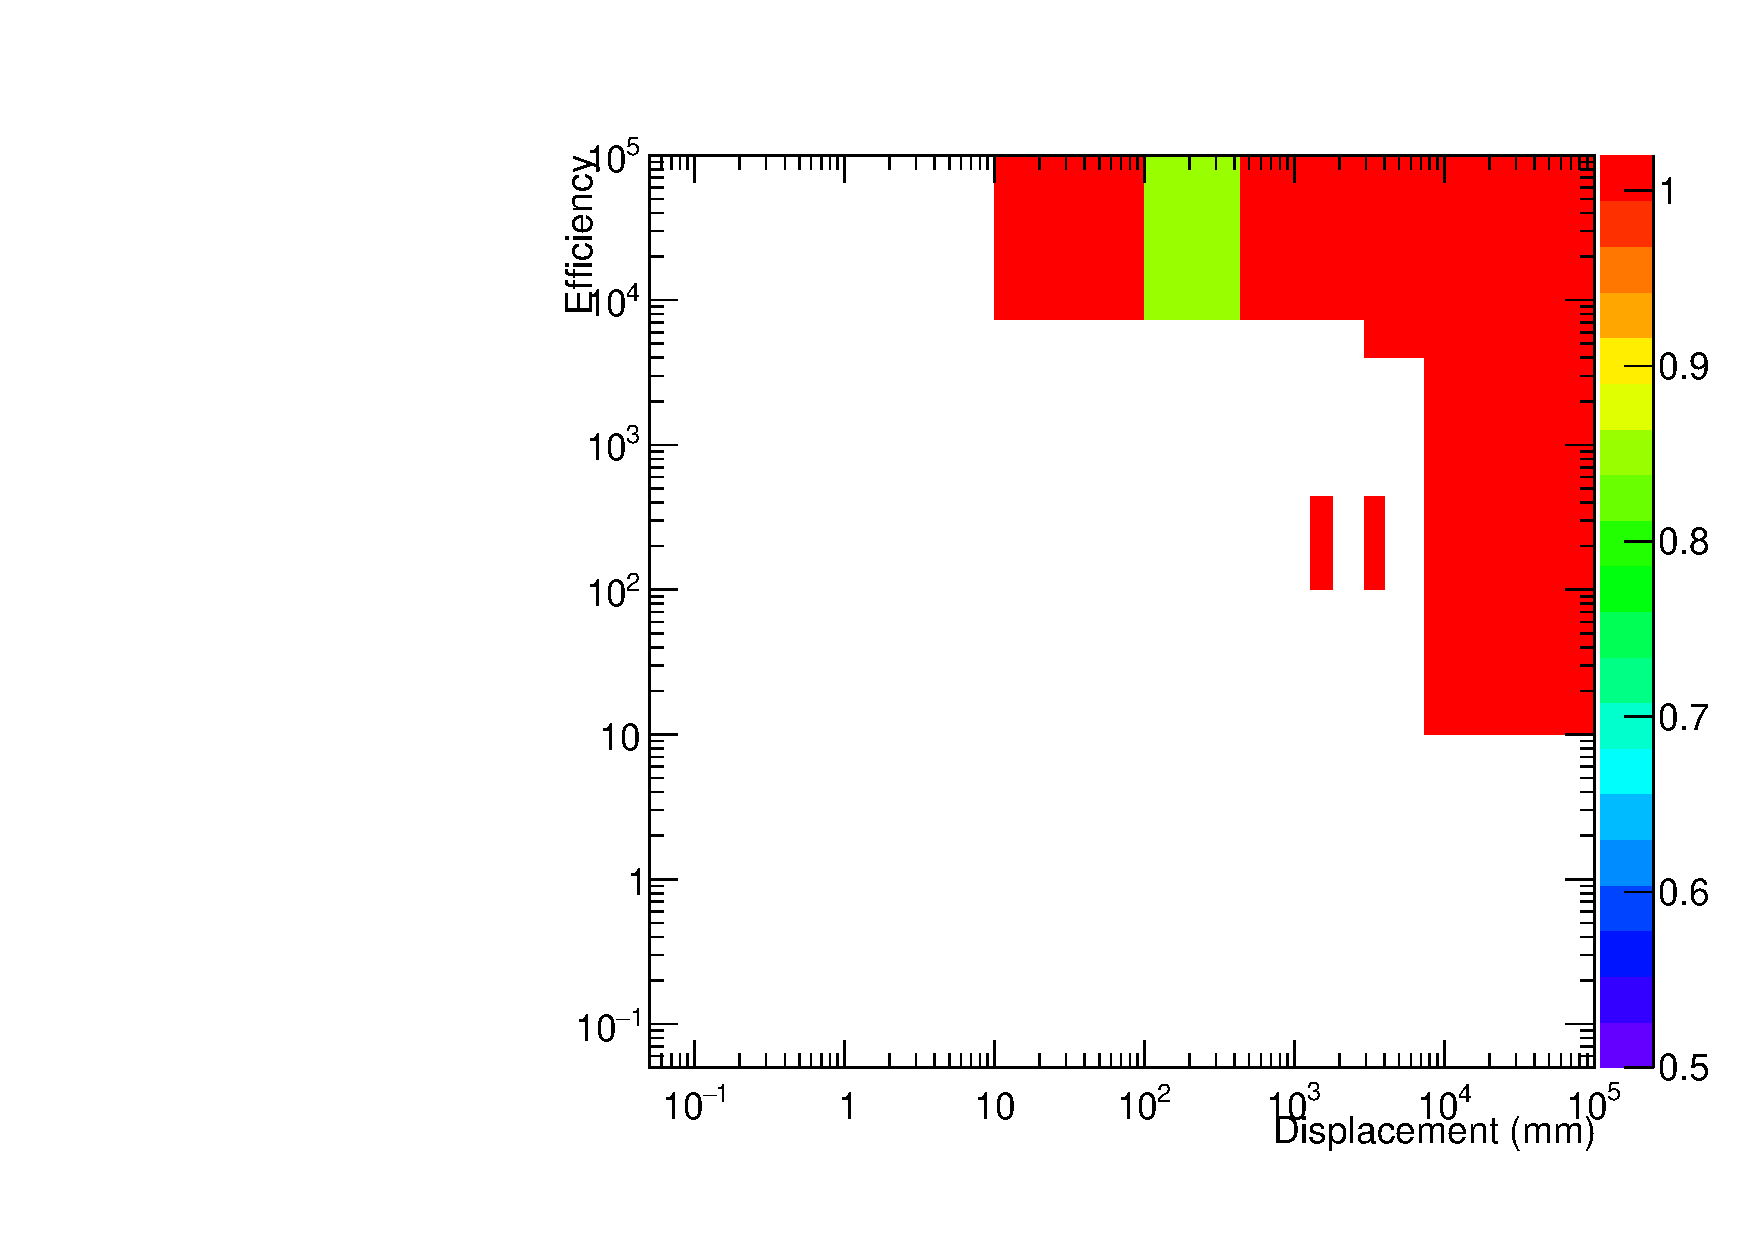
\includegraphics[width=0.4\textwidth]{figures/LLPResults/systs/oddjetveto/Signal_SignalModels__longLivedAnalyzer__SMS-T1qqqqLL_ctau_100000_mGluino-1000_mLSP-200_25ns__eff_oddjet_2D_log_num.pdf} 
    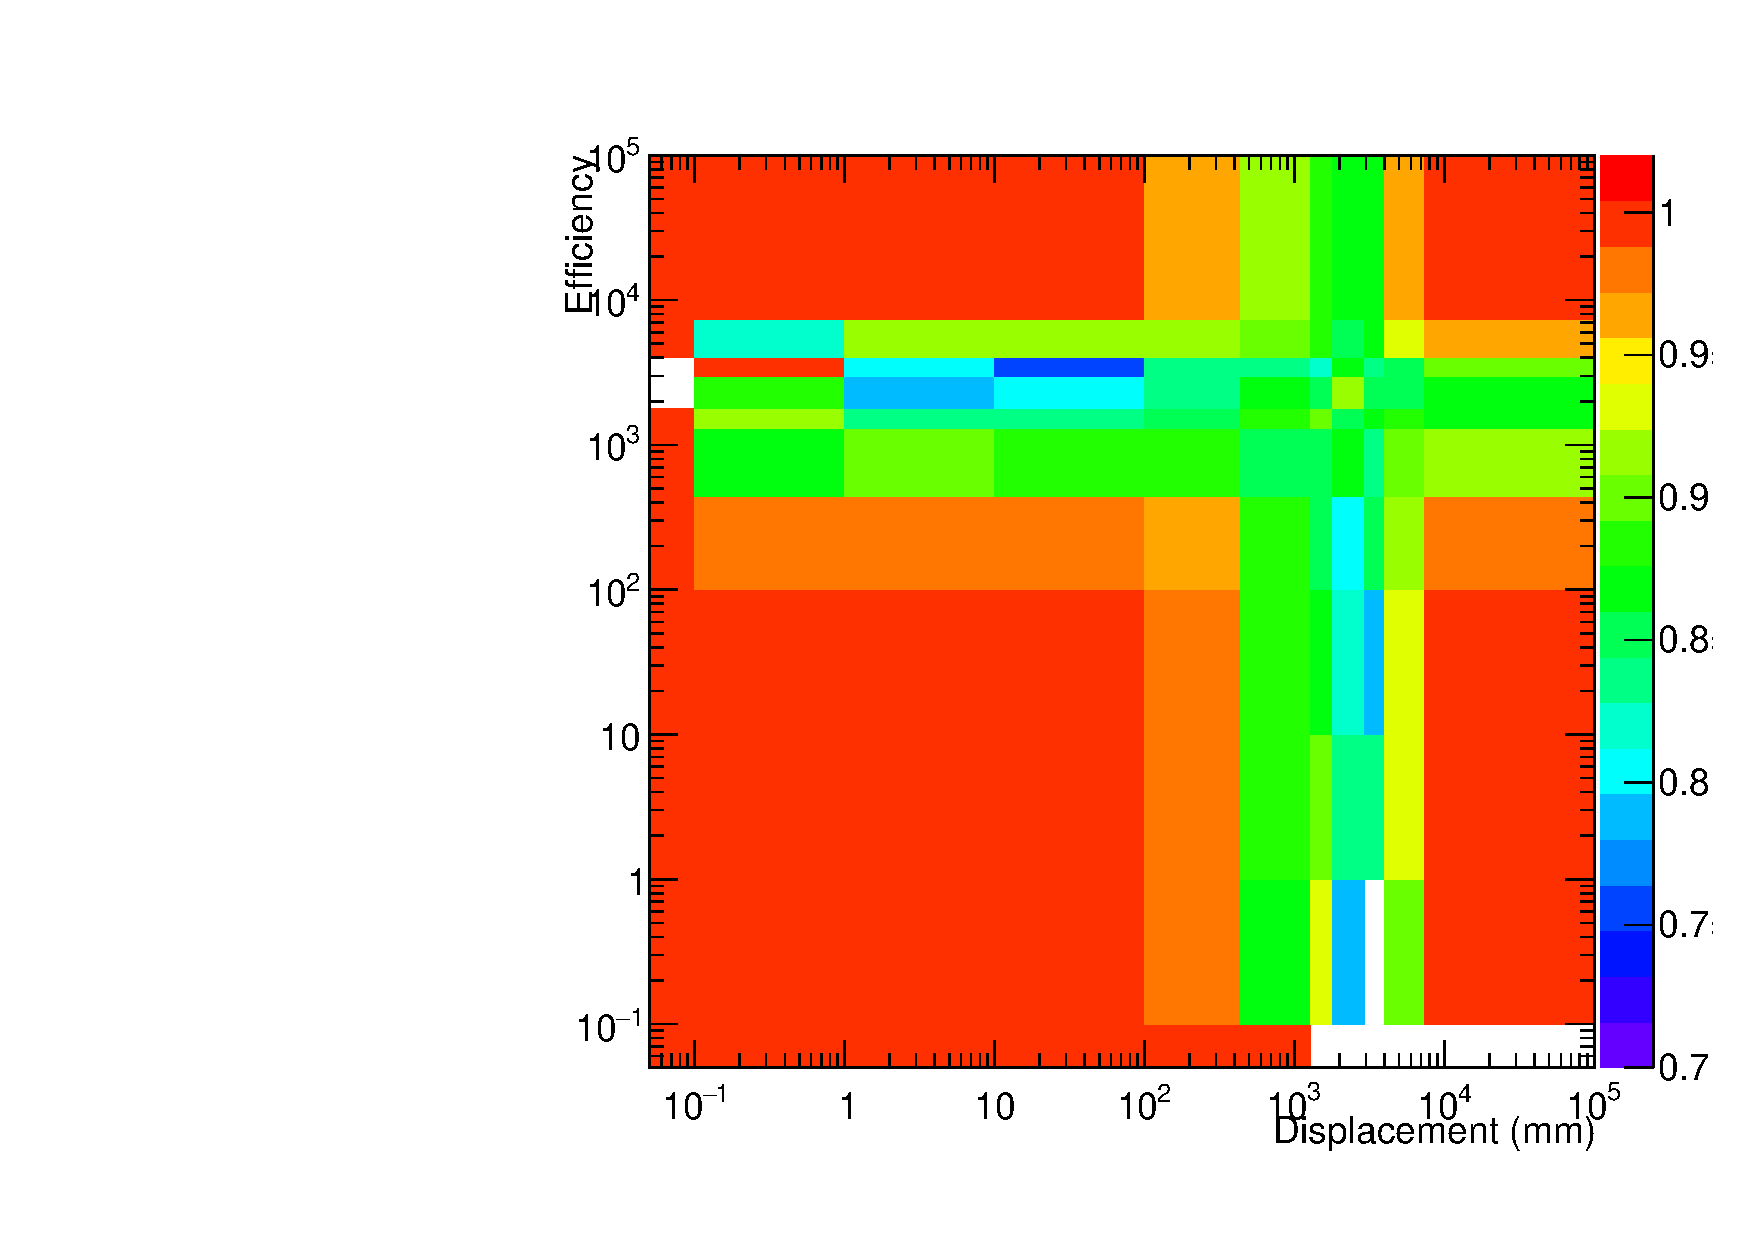
\includegraphics[width=0.4\textwidth]{figures/LLPResults/systs/oddjetveto/Signal_SignalModels__longLivedAnalyzer__SMS_T1qqqqLL_ctau-all__eff_oddjet_2D_log_num.pdf} 
    \caption{Signal efficiency for odd jet veto as a function of the
      flight distances of the each gluino in the event
      (\fixme{incorrect y axis label!}) for the simplified
      \texttt{T1qqqqLL} model for a range of gluino lifetimes,
      $\ctau$: $1\unit{mm}$ (top left), $10\unit{mm}$ (top right),
      $100\unit{mm}$ (centre left), $1000\unit{mm}$ (centre right),
      $10000\unit{mm}$ (bottom left), and $100000\unit{mm}$ (bottom
      right). For illustrative purposes, ``representative''
      efficiencies are also shown when integrating over all models in
      terms of masses and $c\tau$ values (bottom right). }
    \label{fig:oddjetveto}
  \end{center}
\end{figure}

\clearpage
\subsection{Signal trigger efficiencies}
\label{app:LLP-trigger}

Table~\ref{tab:LLP-triggereff} shows the efficiency of the signal
region triggers, listed in Sec.~\ref{sec:triggers}, for the
\texttt{T1qqqqLL} (1800,200), (1000,200), and (1000,900) benchmark
models and as a function of gluino lifetime, $c\tau$.
``Representative'' efficiences as a function of $c\tau$ are also shown
when integrating over all models in terms of masses. Generally, the
trigger efficiency is 100\%, but small inefficiencies of
${\approx}2\%$ are observed for models with $c\tau \gtrsim
10\unit{mm}$, likely due to the \verb!TightID! working point for the
single jet requirement of the monojet trigger. Corrections to the
signal acceptance to account for trigger inefficiencies are determined
from the trigger emulation available within the simulated
samples. Systematic uncertainties of ${\approx}2-3\%$ are taken from
those determined in data, as described in Sec.~\ref{sec:triggers}.

Figure~\ref{fig:triggereffs} shows the signal trigger efficiency as a
function of the flight distances of the each gluino in the event for
the simplified \texttt{T1qqqqLL} model for a range of gluino lifetimes
and the range $10 < \ctau < 100000\unit{mm}$. Any small inefficiencies
tend to be localised to flight distances of either or both gluinos in
the region from ${\approx}100\unit{mm}$ to ${\approx}10\unit{m}$, as
indicated by Figure~\ref{fig:triggereffs} (top left), which shows
``representative'' efficiences when integrating over all masses.

\begin{table}[h!]
  \topcaption{Summary of the signal trigger efficiencies for three
    \texttt{T1qqqqLL} benchmark models ($m_\text{gluino},
    m_\text{LSP}$), as a function of $c\tau$. Also shown are
    ``representative'' efficiences when integrating over all masses.} 
  \centering
  \begin{tabular}{lcccc} 
    \hline
    $c\tau$          & \multicolumn{4}{c}{Efficiency [\%]}               \\
    \cline{2-5}
                     & (1800,200) & (1000,200) & (1000,900) & All masses \\
    \hline
    $0.001\unit{mm}$ & 100.0      & 100.0      & 99.8       & 100.0      \\
%    $0.01\unit{mm}$ & 100.0      & 100.0      & 100.0      & 100.0      \\
    $0.1\unit{mm}$   & 100.0      & 100.0      & 100.0      & 100.0      \\
    $1\unit{mm}$     & 100.0      & 100.0      & 100.0      & 100.0      \\
    $10\unit{mm}$    & 100.0      & 99.6       & 99.4       & 99.3       \\
    $100\unit{mm}$   & 99.9       & 98.7       & 99.7       & 98.2       \\
    $1\unit{m}$      & 100.0      & 97.6       & 99.7       & 98.0       \\
    $10\unit{m}$     & 97.9       & 98.4       & 99.5       & 98.3       \\
    $100\unit{m}$    & --         & 99.8       & 100.0      & 99.6       \\
    \hline
  \end{tabular}
  \label{tab:LLP-triggereff}
\end{table}

\begin{figure}[h!]
  \begin{center}
%    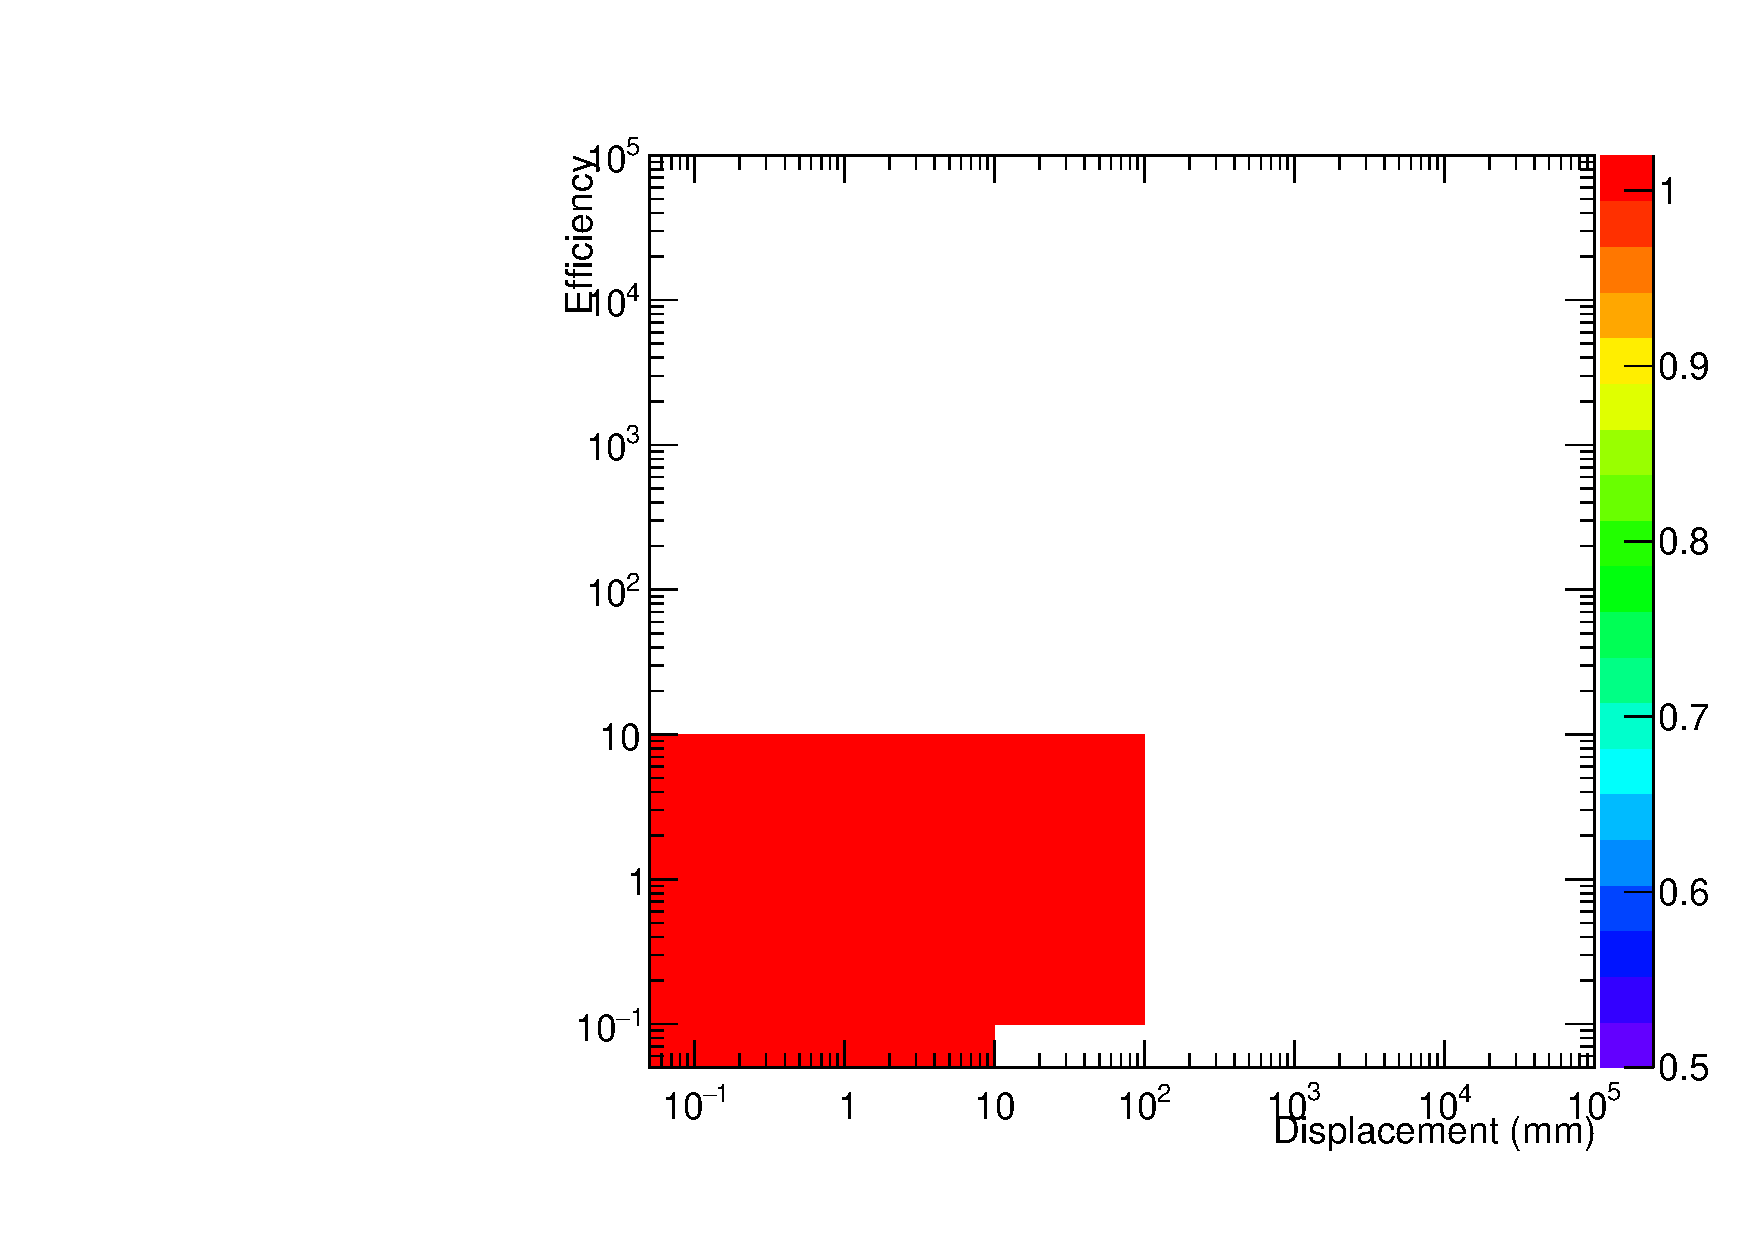
\includegraphics[width=0.4\textwidth]{figures/LLPResults/systs/trigger/Signal_SignalModels__longLivedAnalyzer__SMS-T1qqqqLL_ctau_1_mGluino-1000_mLSP-200_25ns__eff_trigger_2D_log_num.pdf} 
    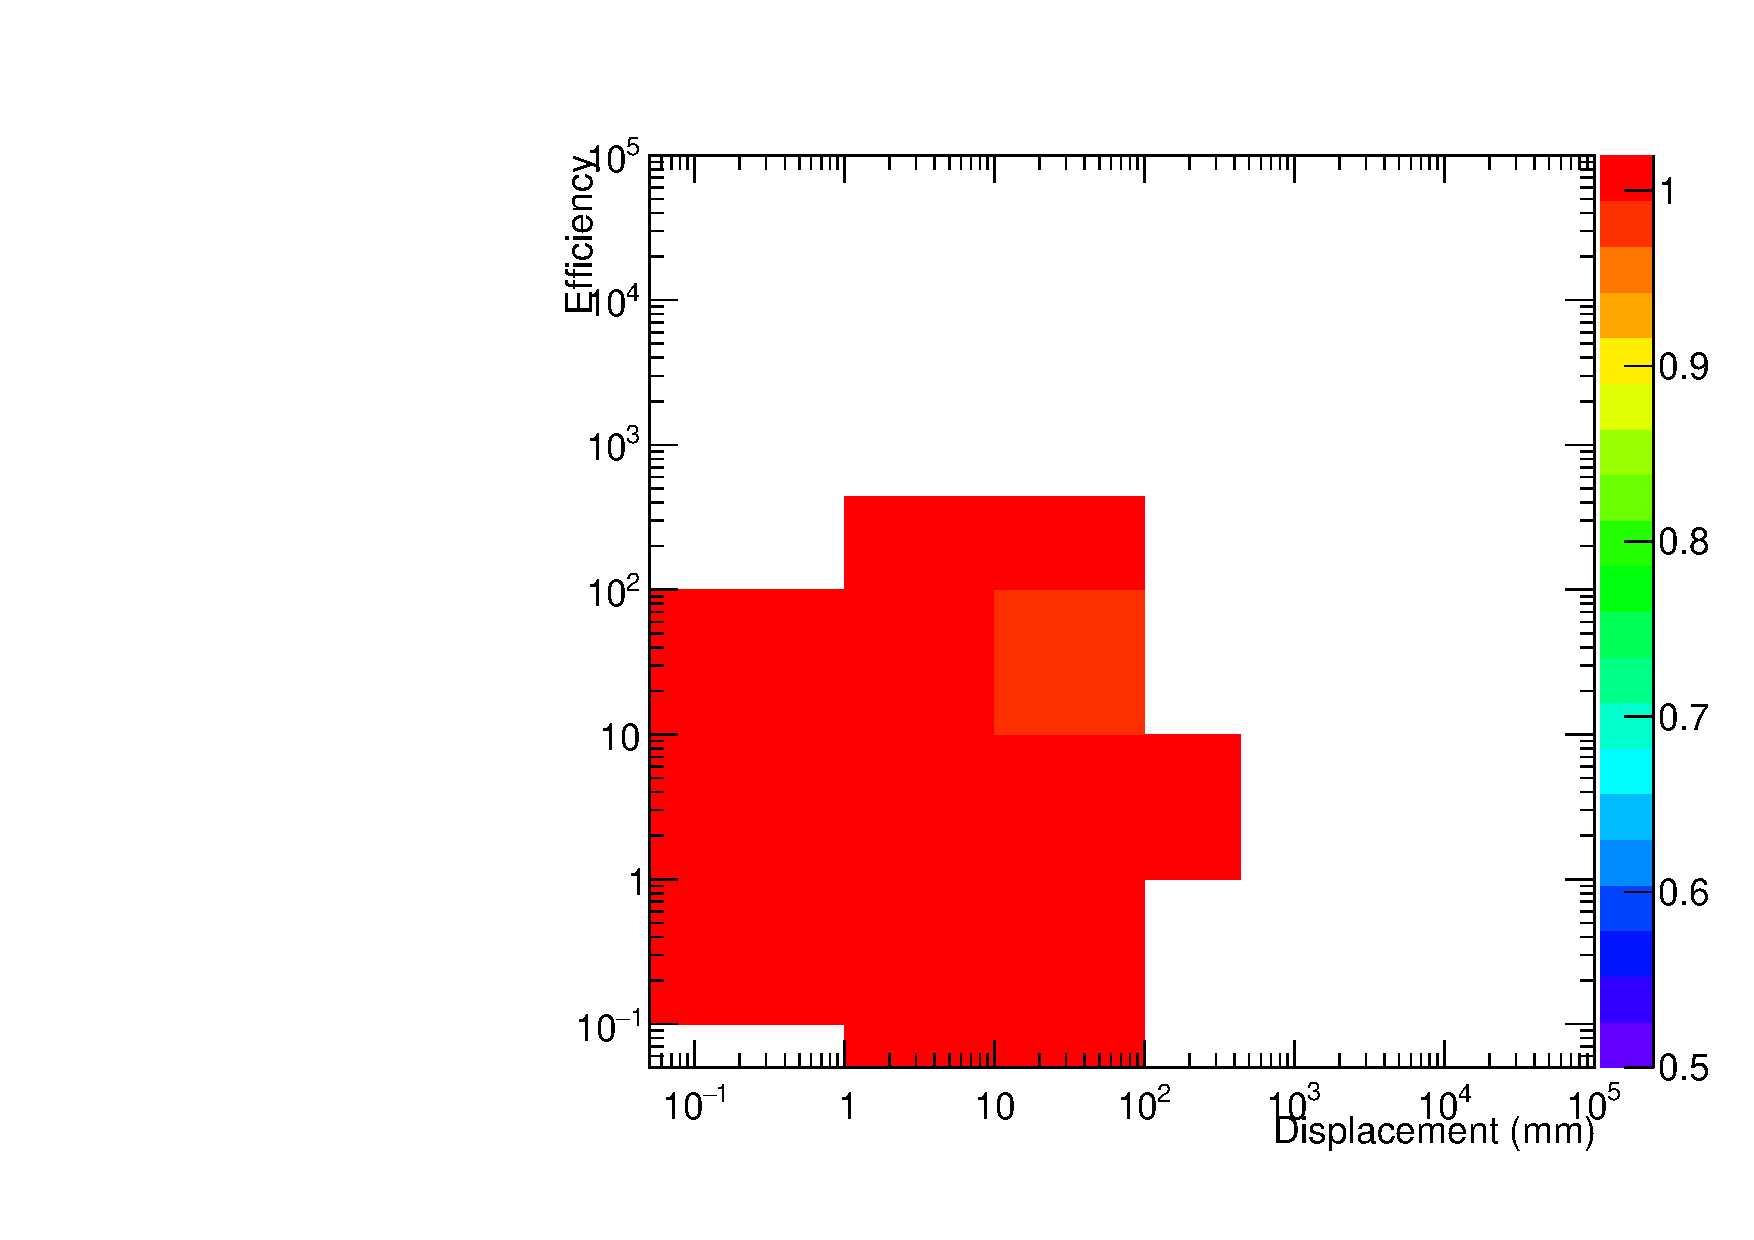
\includegraphics[width=0.4\textwidth]{figures/LLPResults/systs/trigger/Signal_SignalModels__longLivedAnalyzer__SMS-T1qqqqLL_ctau_10_mGluino-1000_mLSP-200_25ns__eff_trigger_2D_log_num.pdf} 
    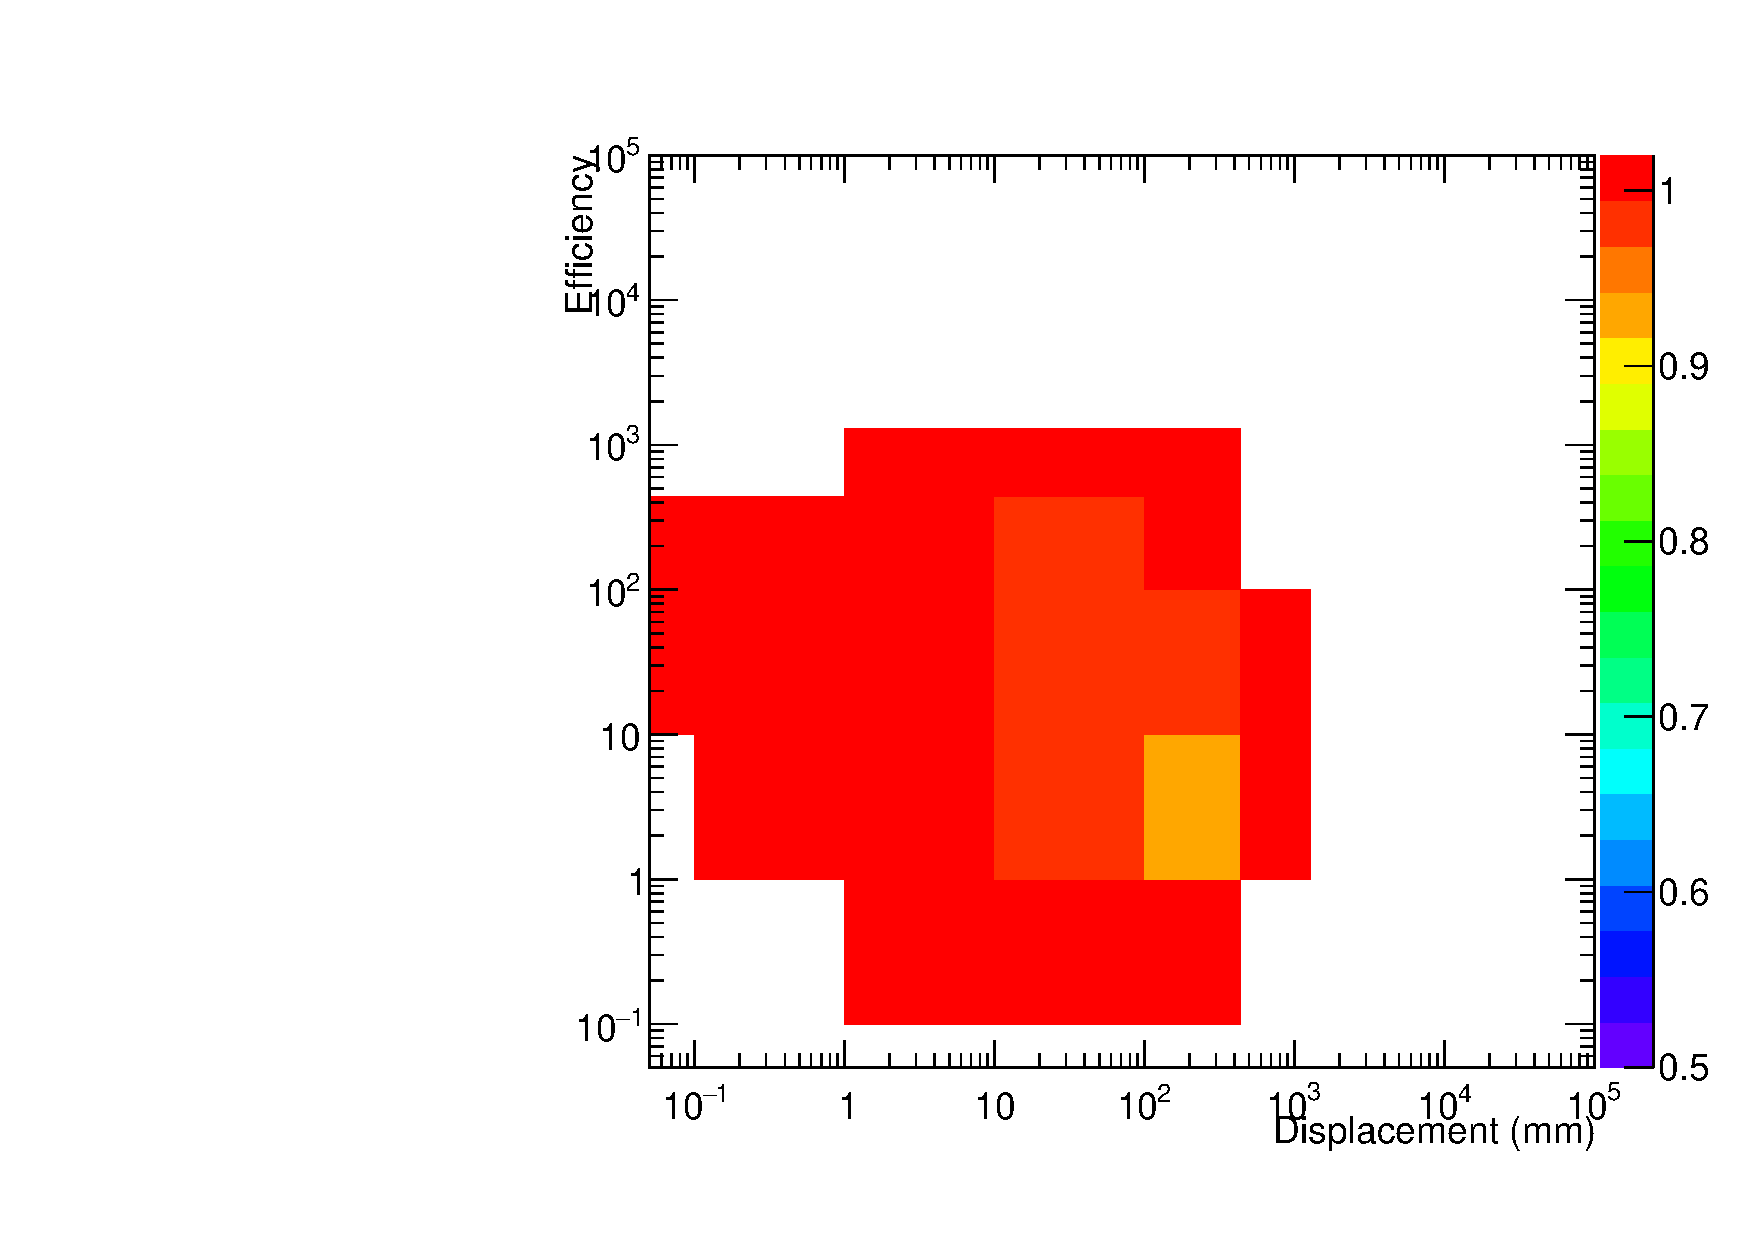
\includegraphics[width=0.4\textwidth]{figures/LLPResults/systs/trigger/Signal_SignalModels__longLivedAnalyzer__SMS-T1qqqqLL_ctau_100_mGluino-1000_mLSP-200_25ns__eff_trigger_2D_log_num.pdf} \\
    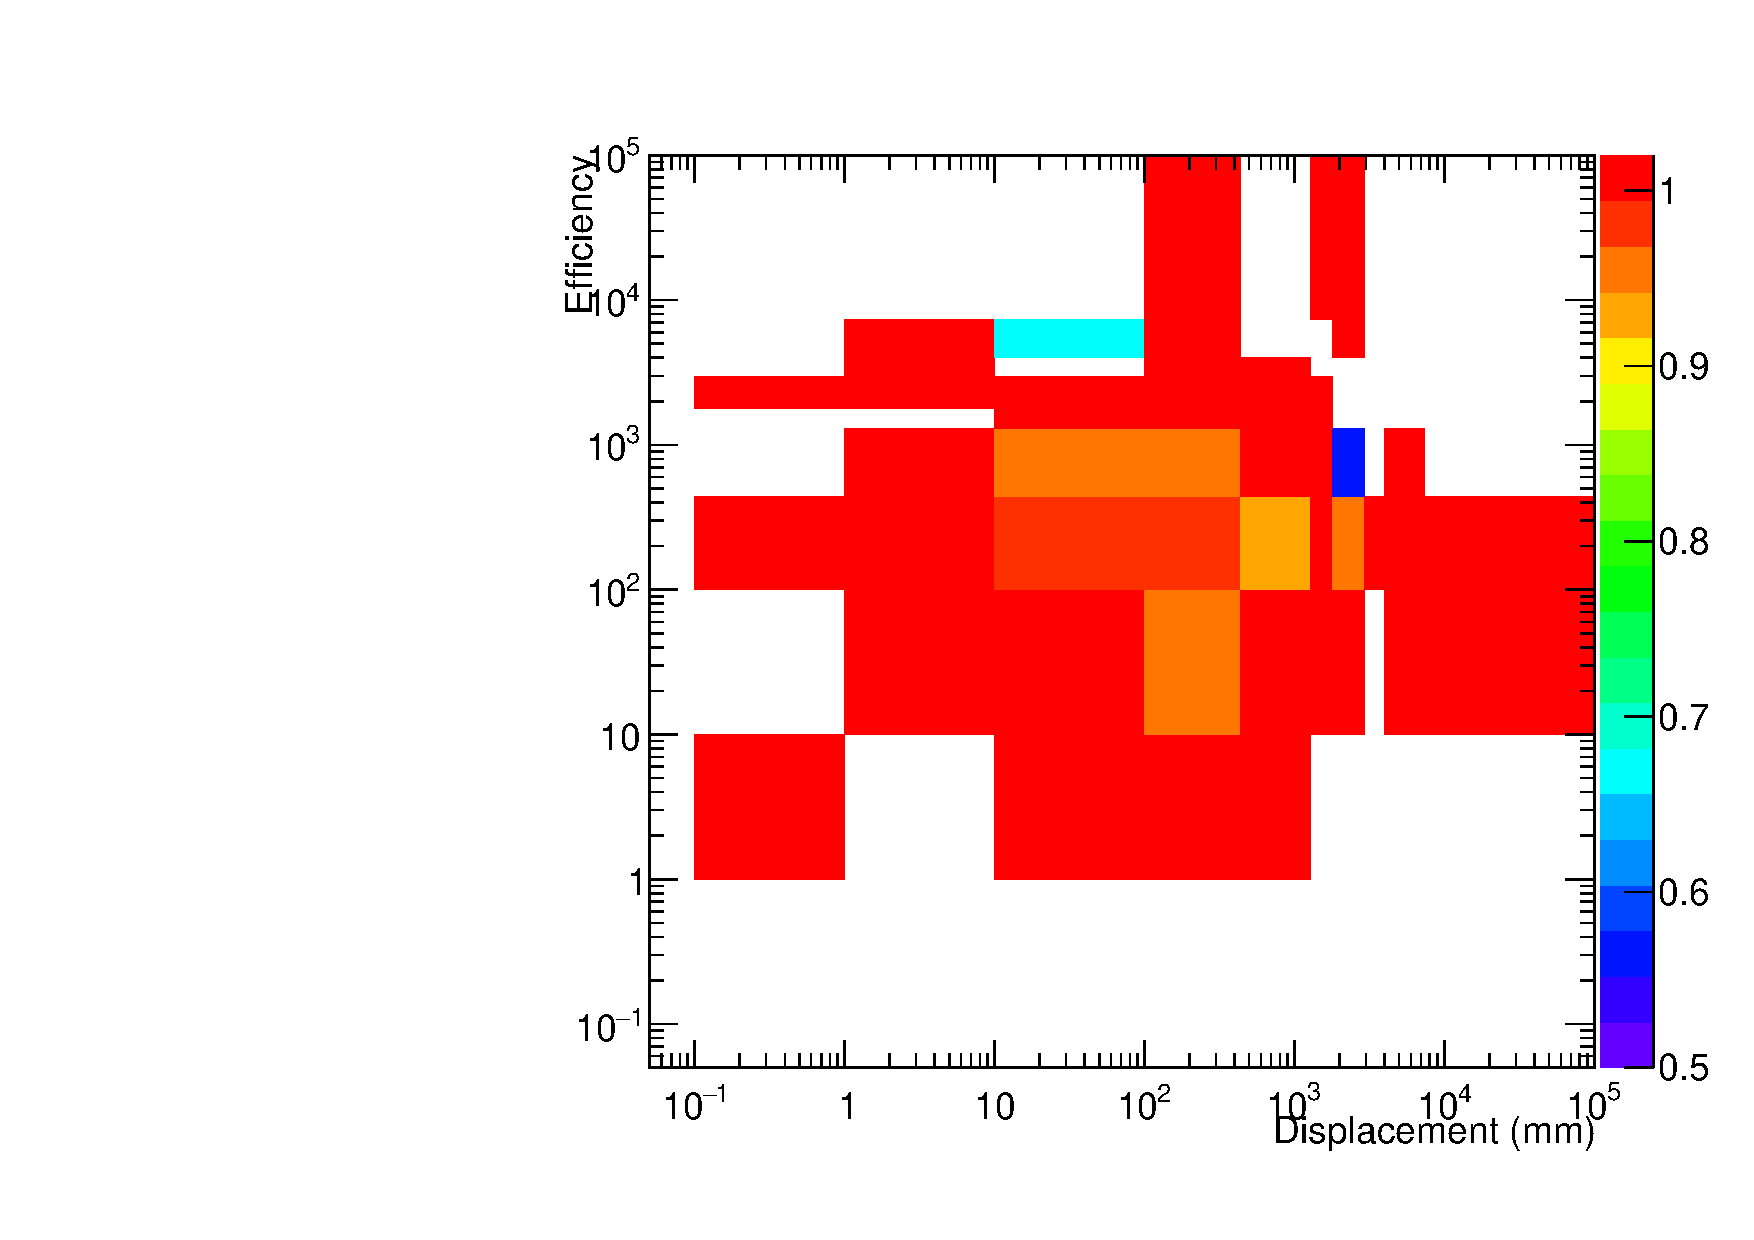
\includegraphics[width=0.4\textwidth]{figures/LLPResults/systs/trigger/Signal_SignalModels__longLivedAnalyzer__SMS-T1qqqqLL_ctau_1000_mGluino-1000_mLSP-200_25ns__eff_trigger_2D_log_num.pdf} 
    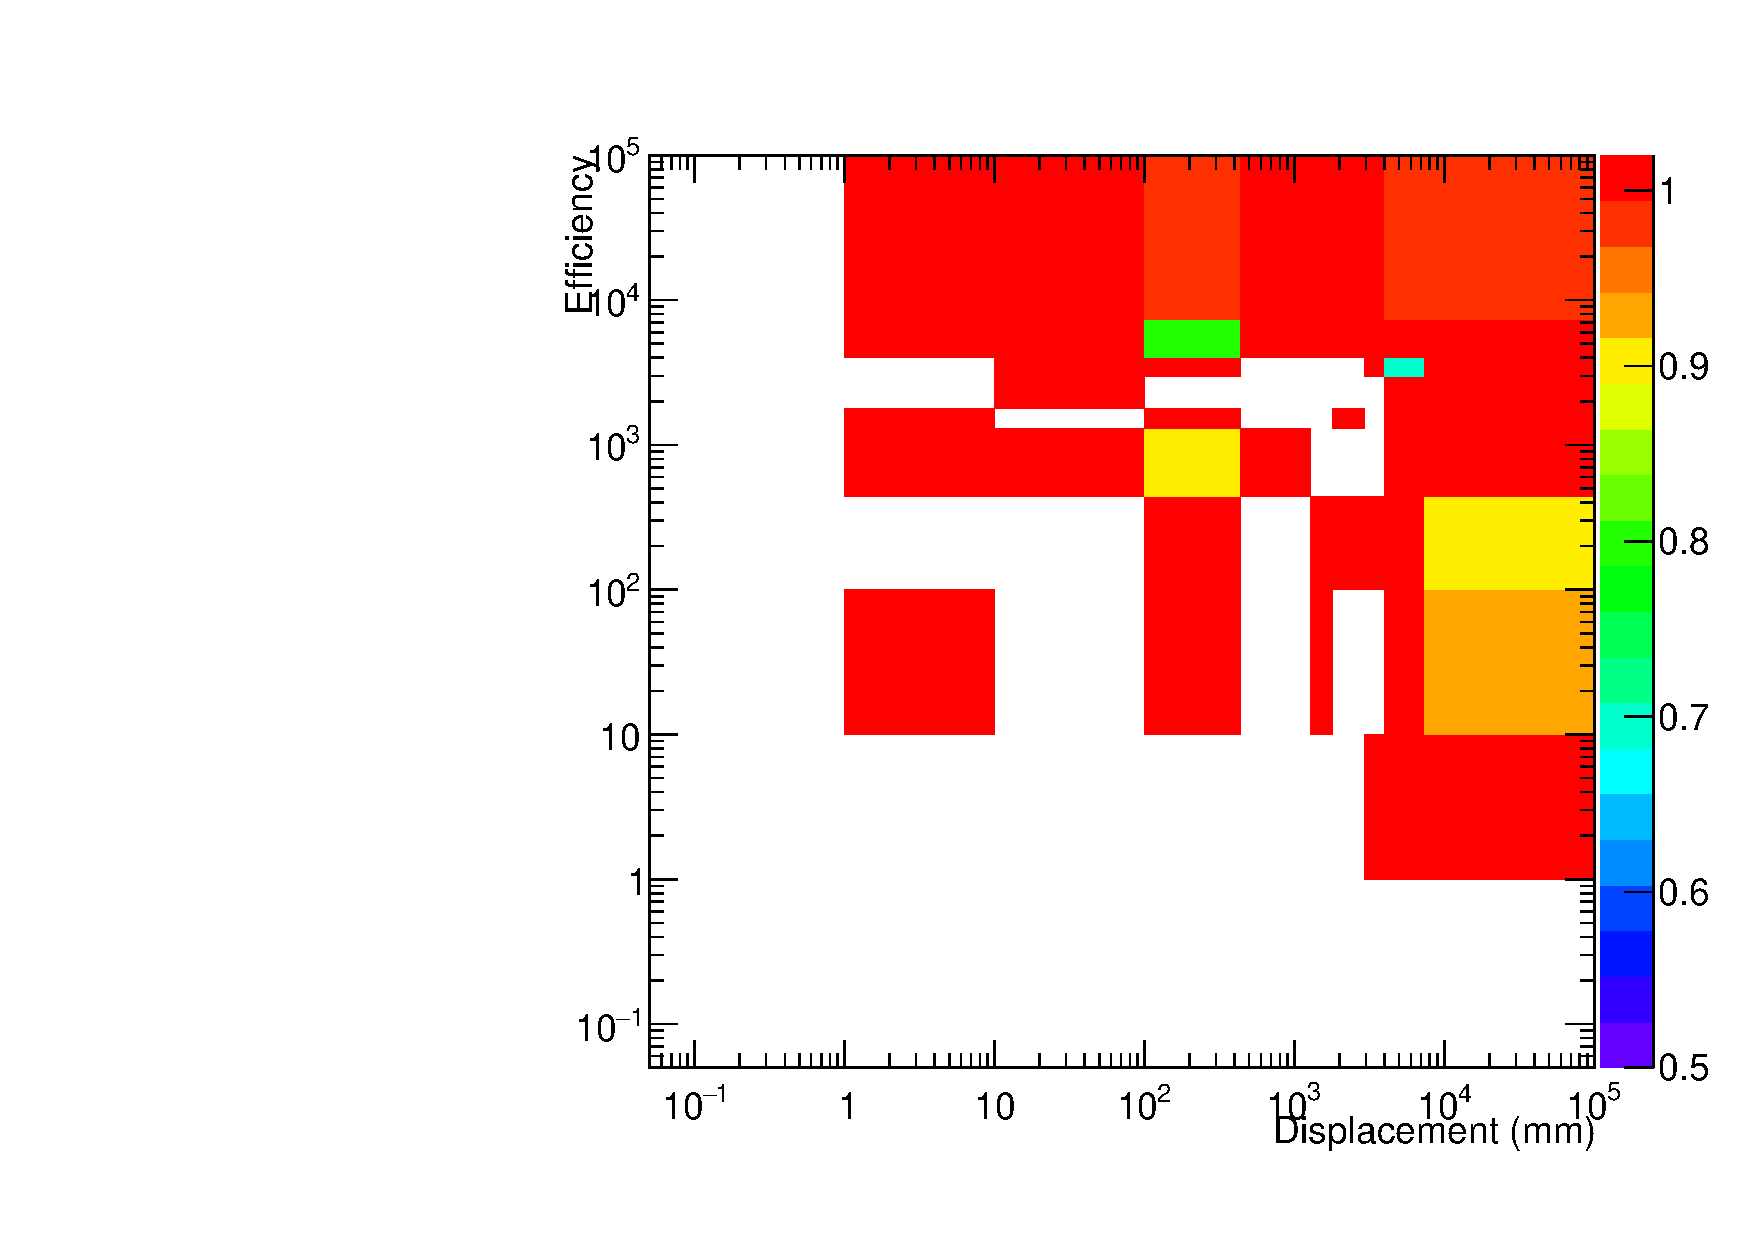
\includegraphics[width=0.4\textwidth]{figures/LLPResults/systs/trigger/Signal_SignalModels__longLivedAnalyzer__SMS-T1qqqqLL_ctau_10000_mGluino-1000_mLSP-200_25ns__eff_trigger_2D_log_num.pdf} \\
    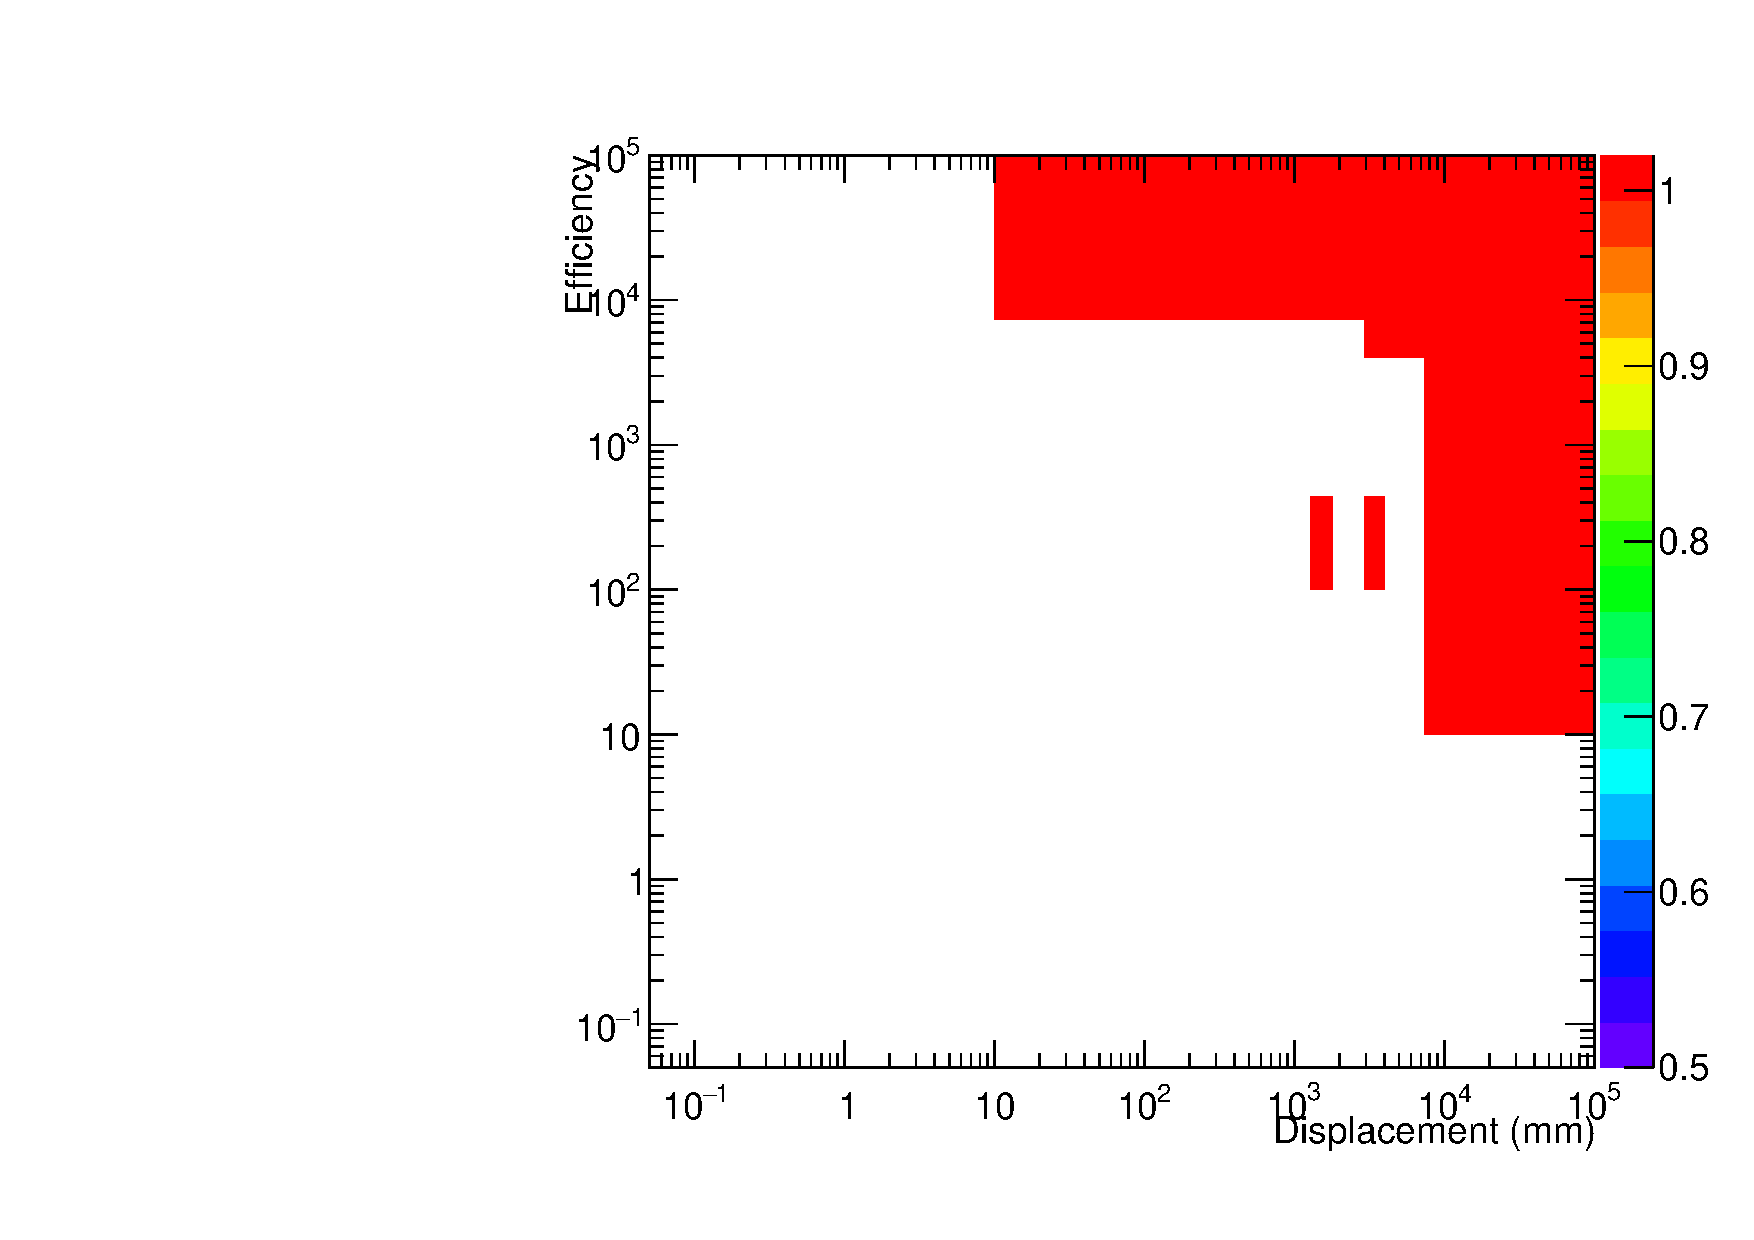
\includegraphics[width=0.4\textwidth]{figures/LLPResults/systs/trigger/Signal_SignalModels__longLivedAnalyzer__SMS-T1qqqqLL_ctau_100000_mGluino-1000_mLSP-200_25ns__eff_trigger_2D_log_num.pdf} 
    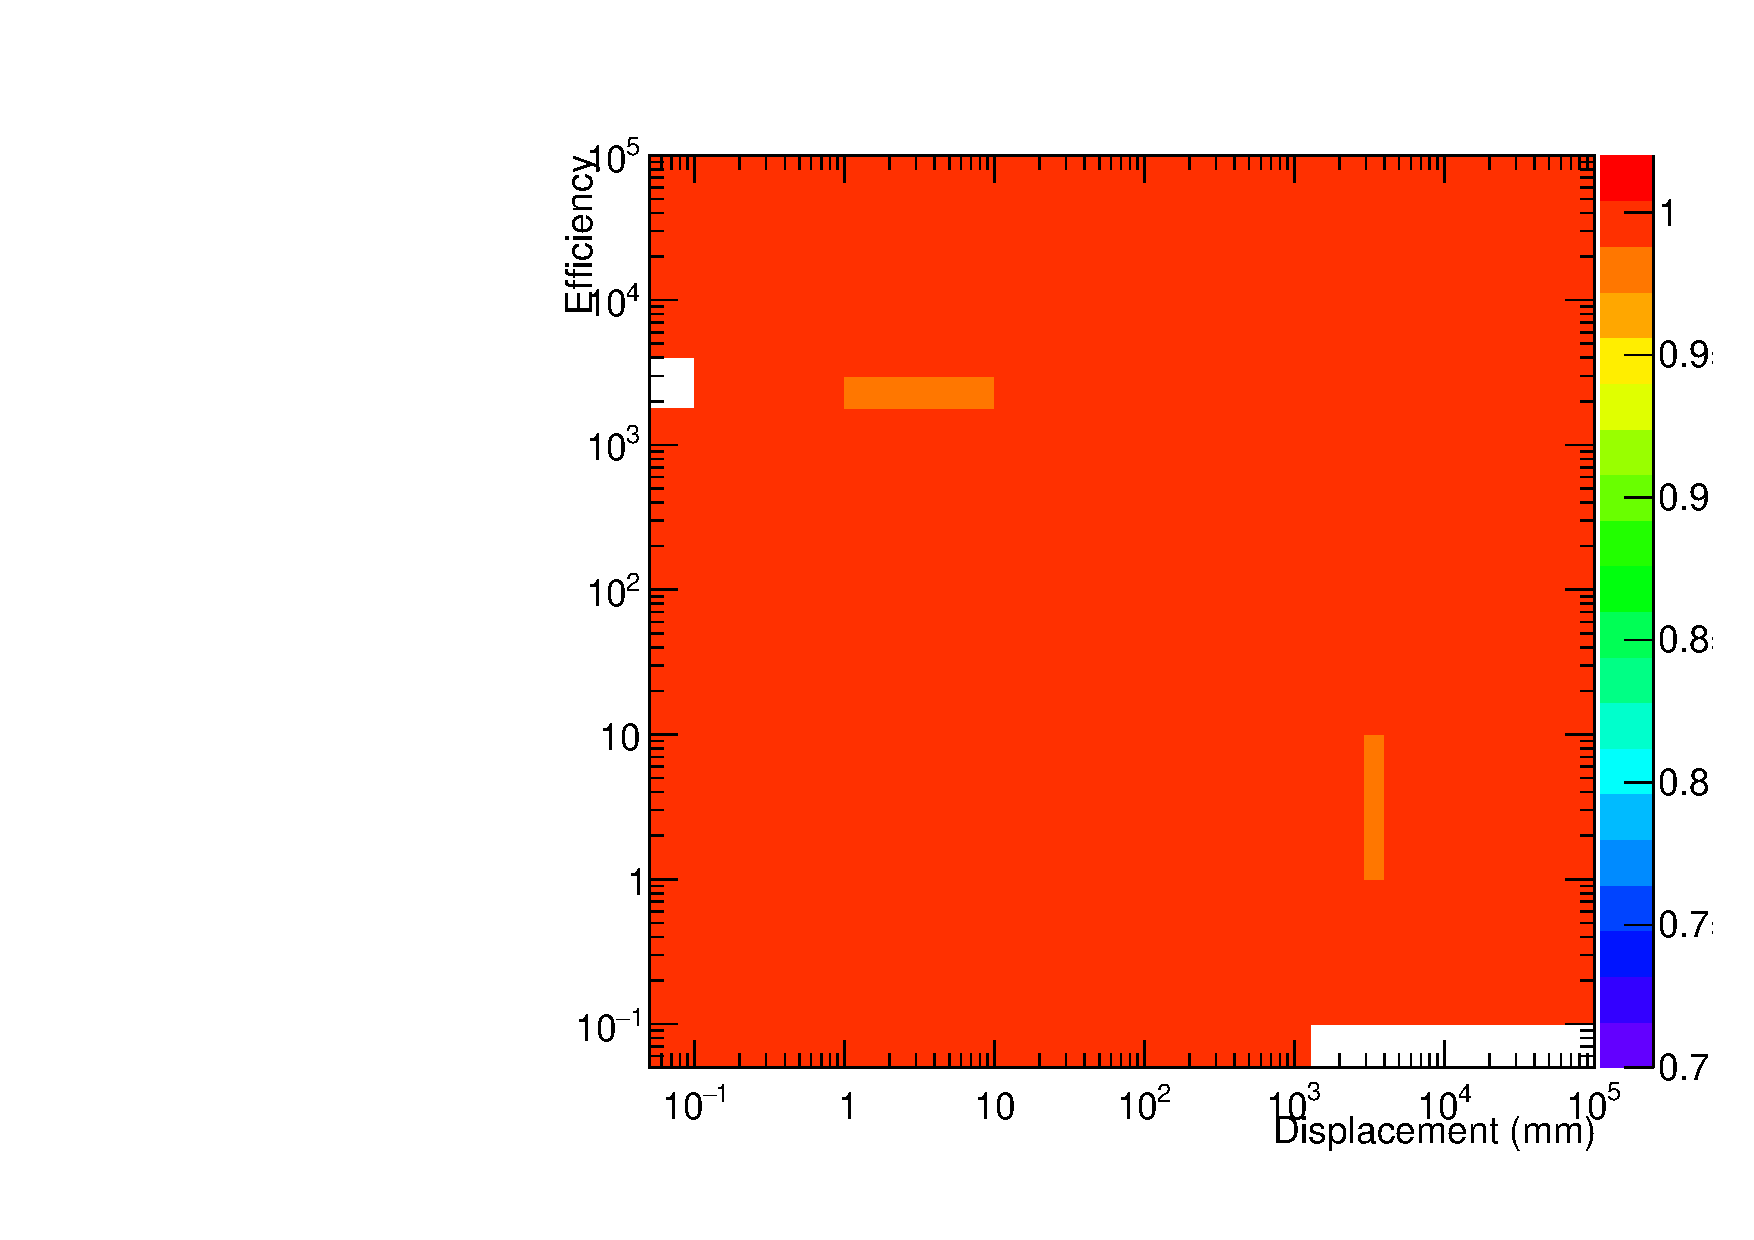
\includegraphics[width=0.4\textwidth]{figures/LLPResults/systs/trigger/Signal_SignalModels__longLivedAnalyzer__SMS_T1qqqqLL_ctau-all__eff_trigger_2D_log_num.pdf} 
    \caption{Trigger efficiency as a function of the flight distances
      of the each gluino in the event (\fixme{incorrect y axis
        label!}) for the simplified \texttt{T1qqqqLL} model for a
      range of gluino lifetimes, $\ctau$: $10\unit{mm}$ (top left),
      $100\unit{mm}$ (top right), $1000\unit{mm}$ (centre left),
      $10000\unit{mm}$ (centre right), and $100000\unit{mm}$ (bottom
      left). For illustrative purposes, ``representative''
      efficiencies are also shown when integrating over all models in
      terms of masses and $c\tau$ values (bottom right).  }
    \label{fig:triggereffs}
  \end{center}
\end{figure}

\clearpage
\subsection{Jet response}
\label{app:LLP-jetresponse}

Figure~\ref{fig:T1qqqq:response} shows the jet response (defined as
the ratio of reconstructed \pt to generator-level \pt) for generator
jets with $\pt>40$ and $|\eta|<2.4$ for the different lifetimes
considered.

\begin{figure}
  \begin{center}
    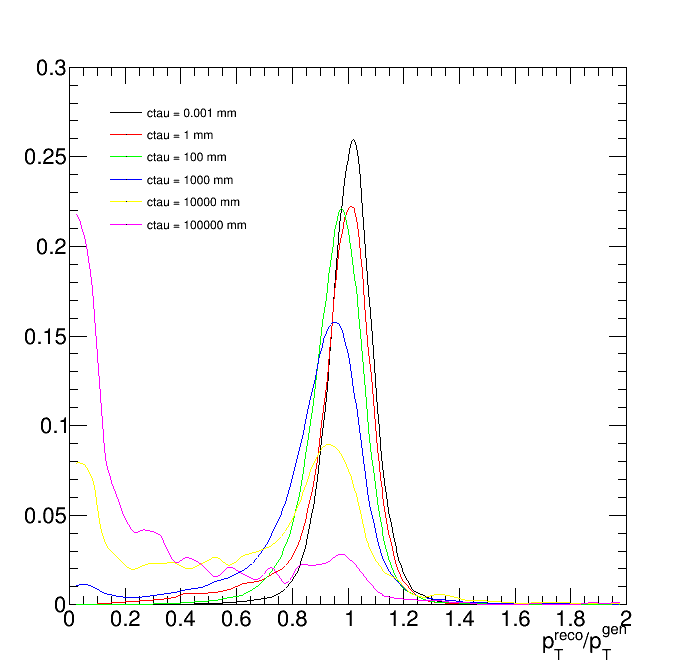
\includegraphics[width=0.6\textwidth]{figures/LLPResults/T1qqqqLL_response}
    \caption{Distribution of response for generator-level jets with
      $\pt>40$ and $|\eta|<2.4$, for various \ctau models. Only jets
      originating from one of the long-lived gluinos and that are
      matched to a reconstructed jet are considered.}
    \label{fig:T1qqqq:response}
  \end{center}
\end{figure}

\subsection{b-tagging}
\label{app:LLP-btagging}

Documentation in progress. See slides and email exchange with BTV on the
hypernews for the agreement that was reached in terms of b-tag scale factors 
and associated uncertainties.

